\title{PCB Analysis}

\date{\today}

\documentclass[12pt]{article}

\usepackage{graphicx}

\begin{document}
\maketitle

\section{Volume Analysis Setup}
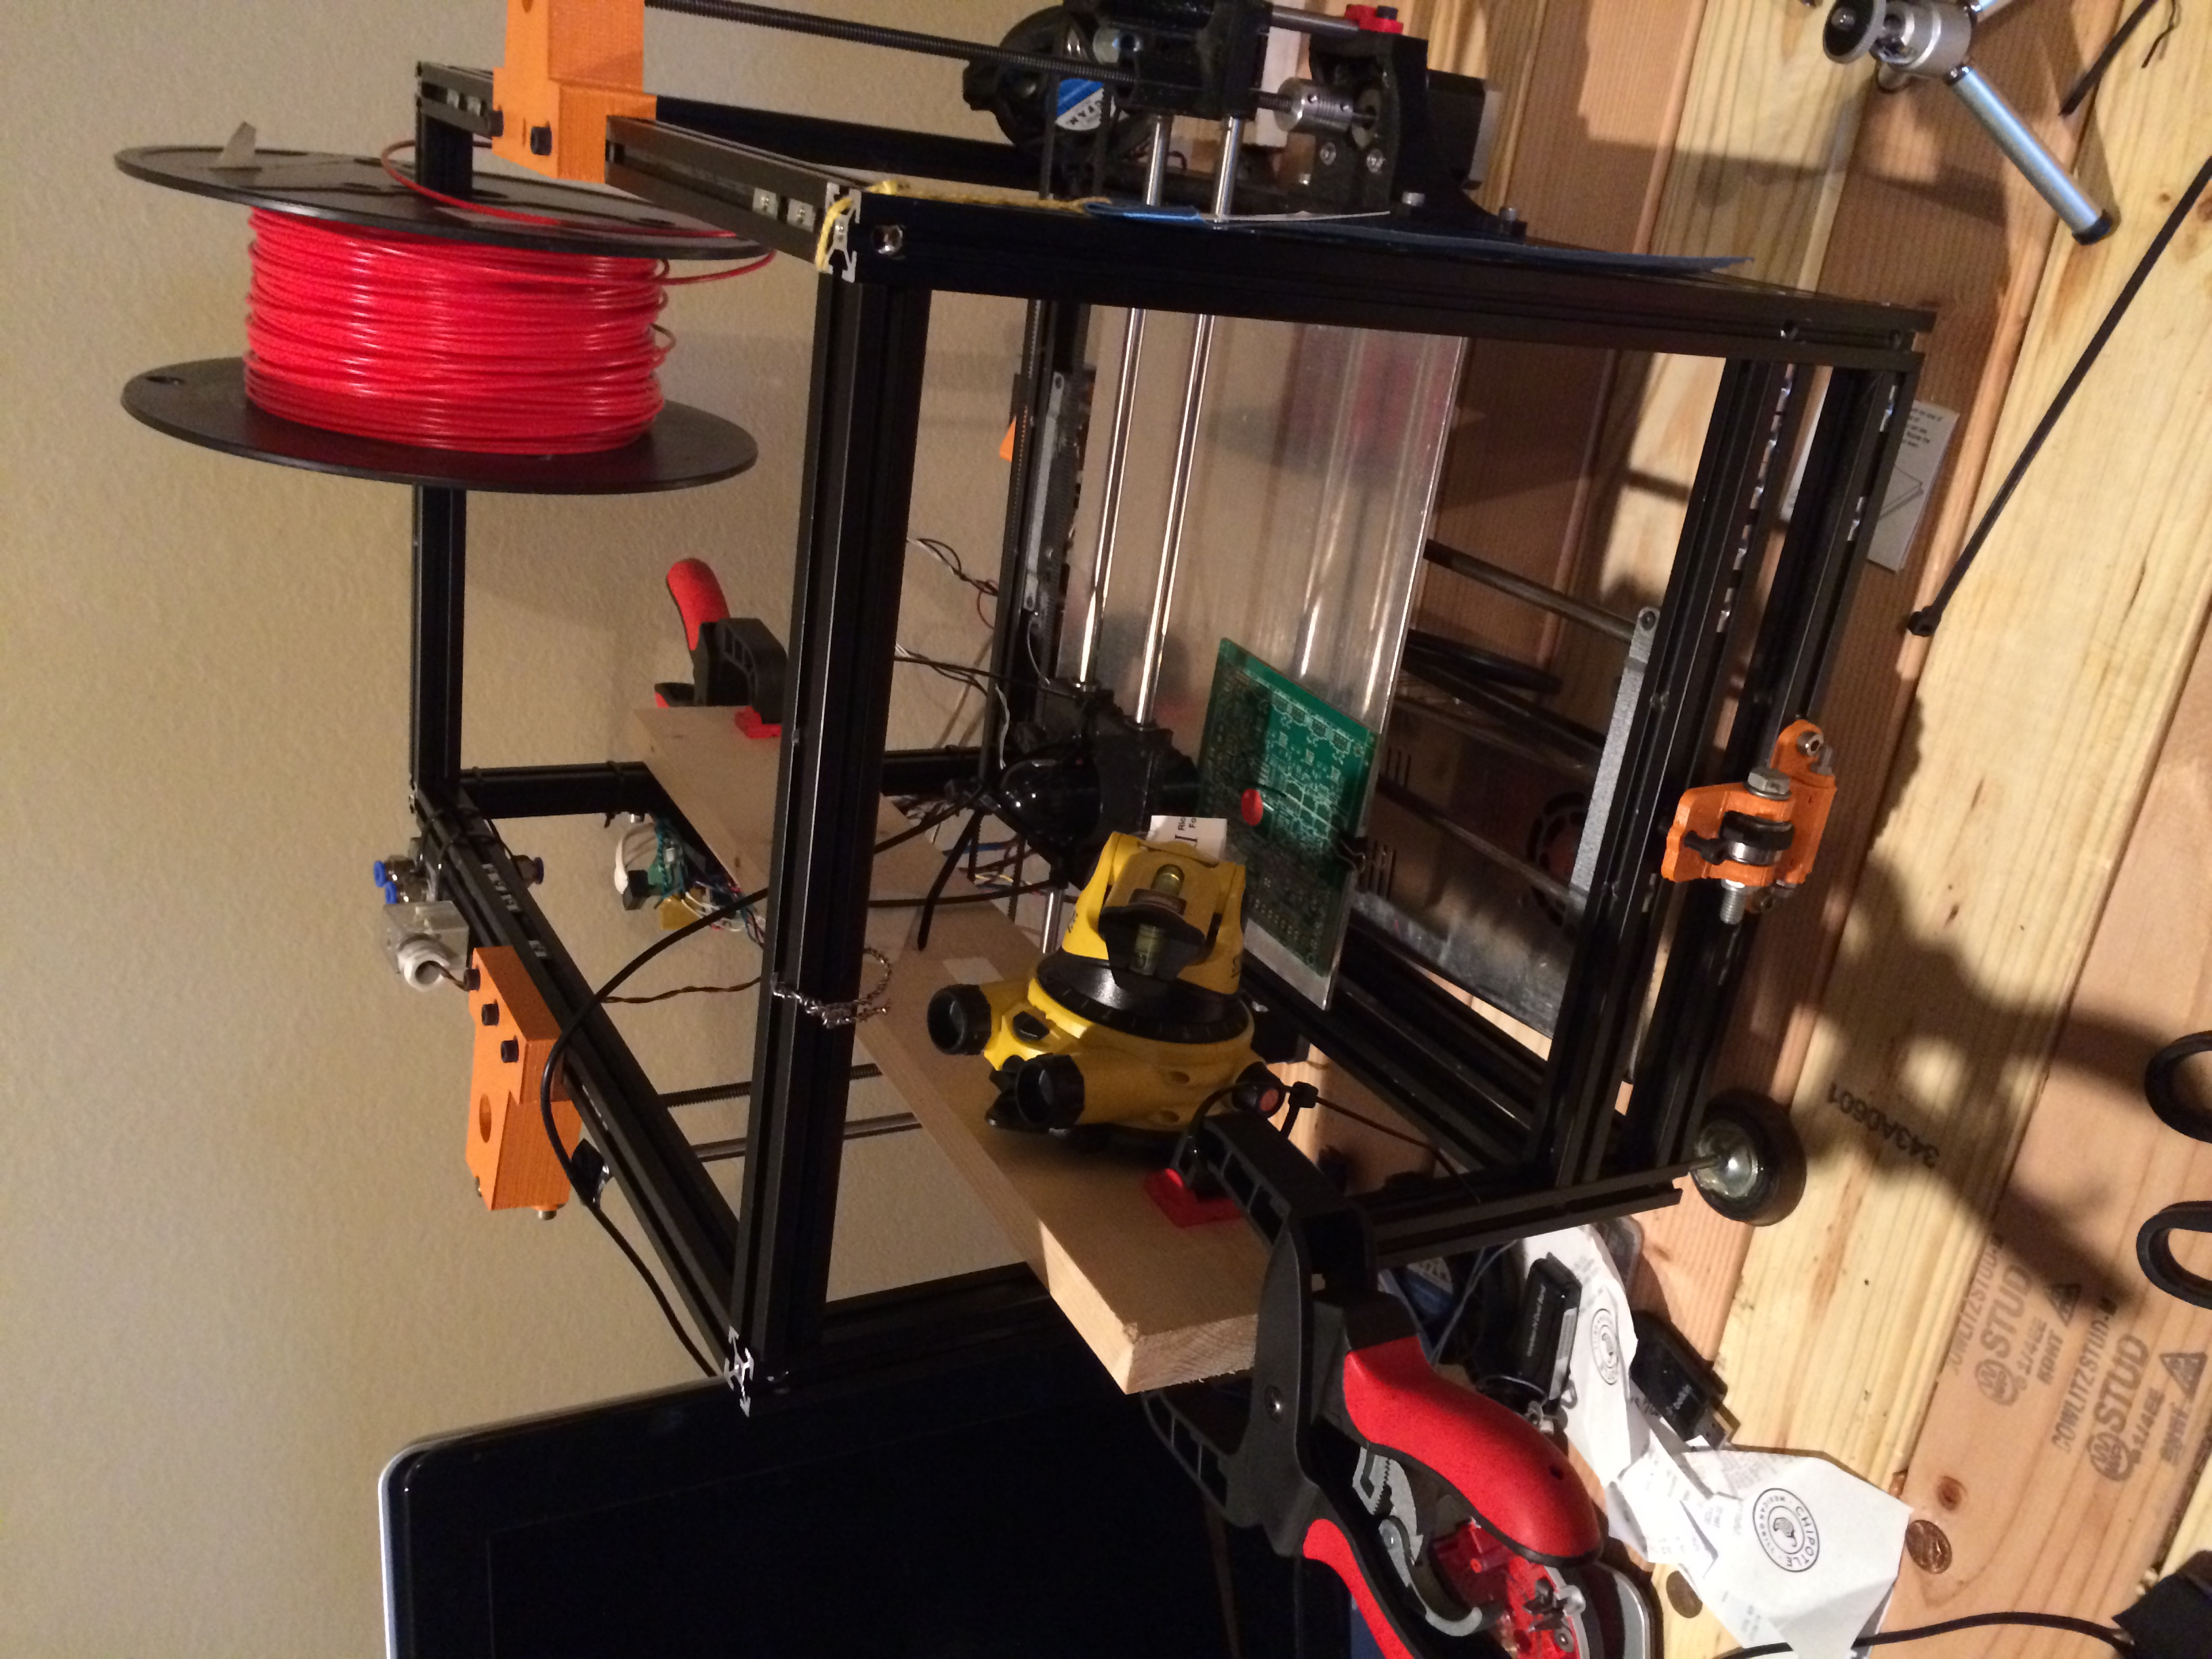
\includegraphics[scale=0.1,angle=270]{images/volume_analysis_setup/IMG_0604.JPG}
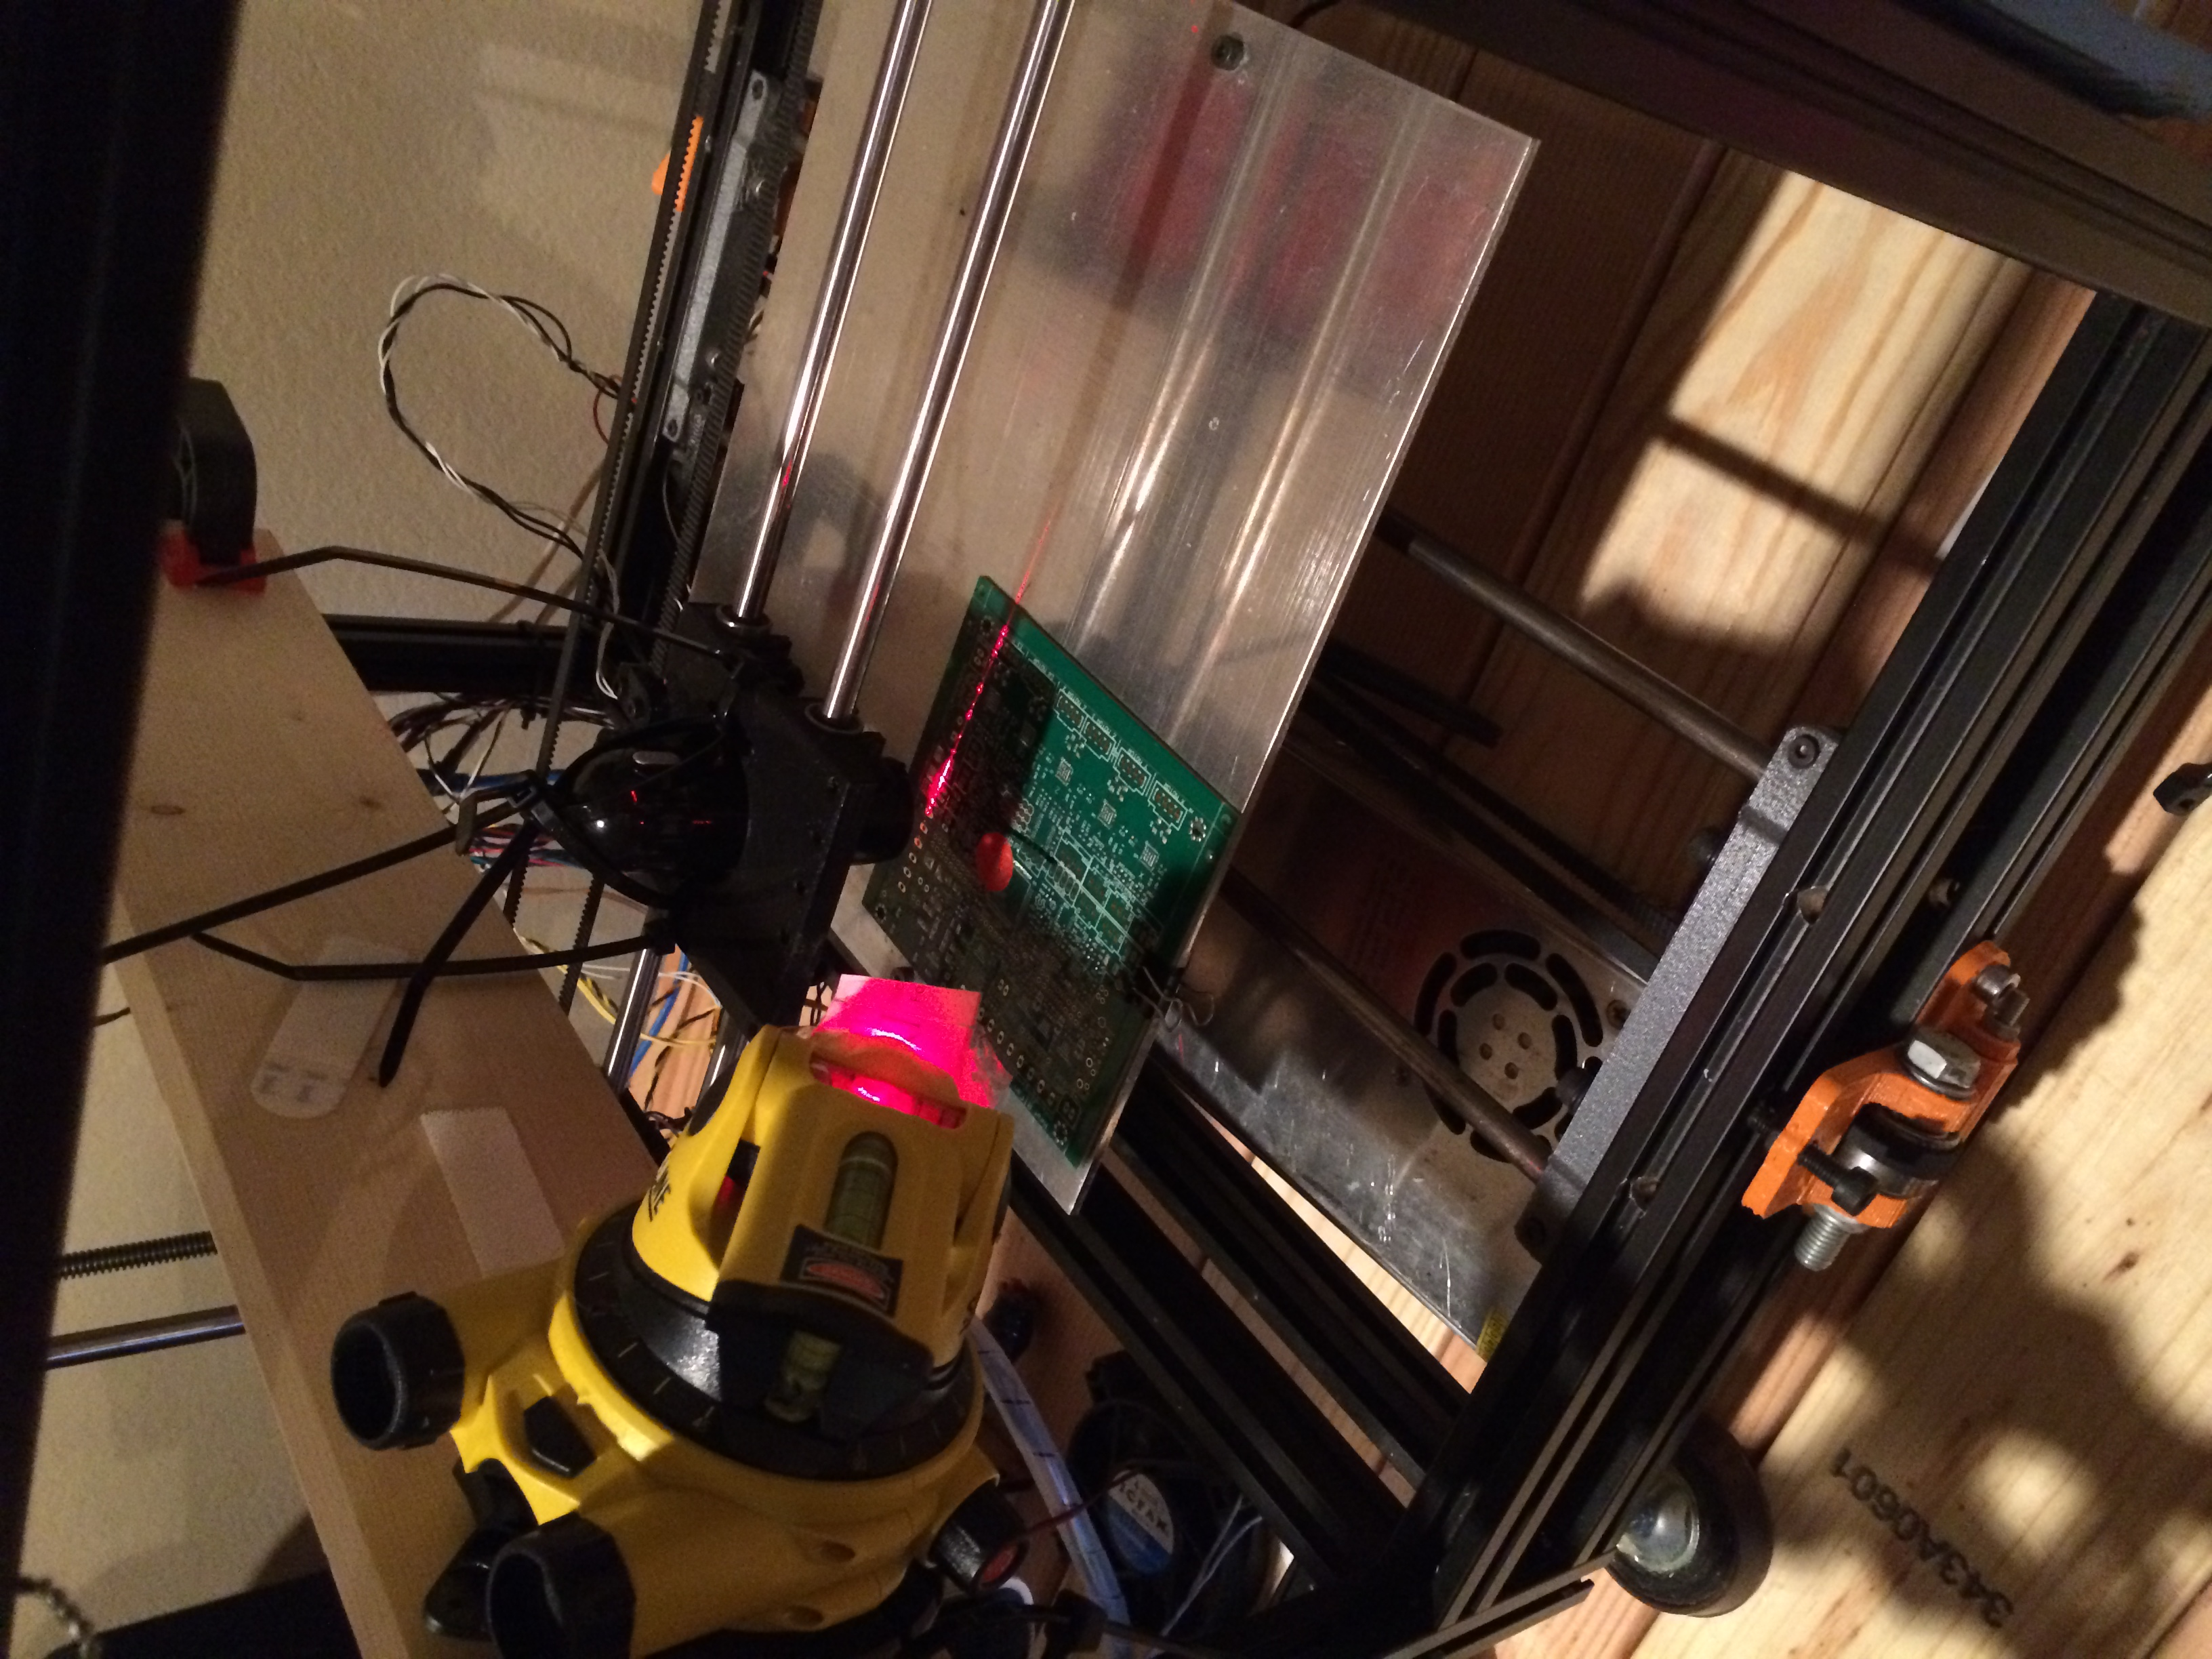
\includegraphics[scale=0.1,angle=270]{images/volume_analysis_setup/IMG_0605.JPG}
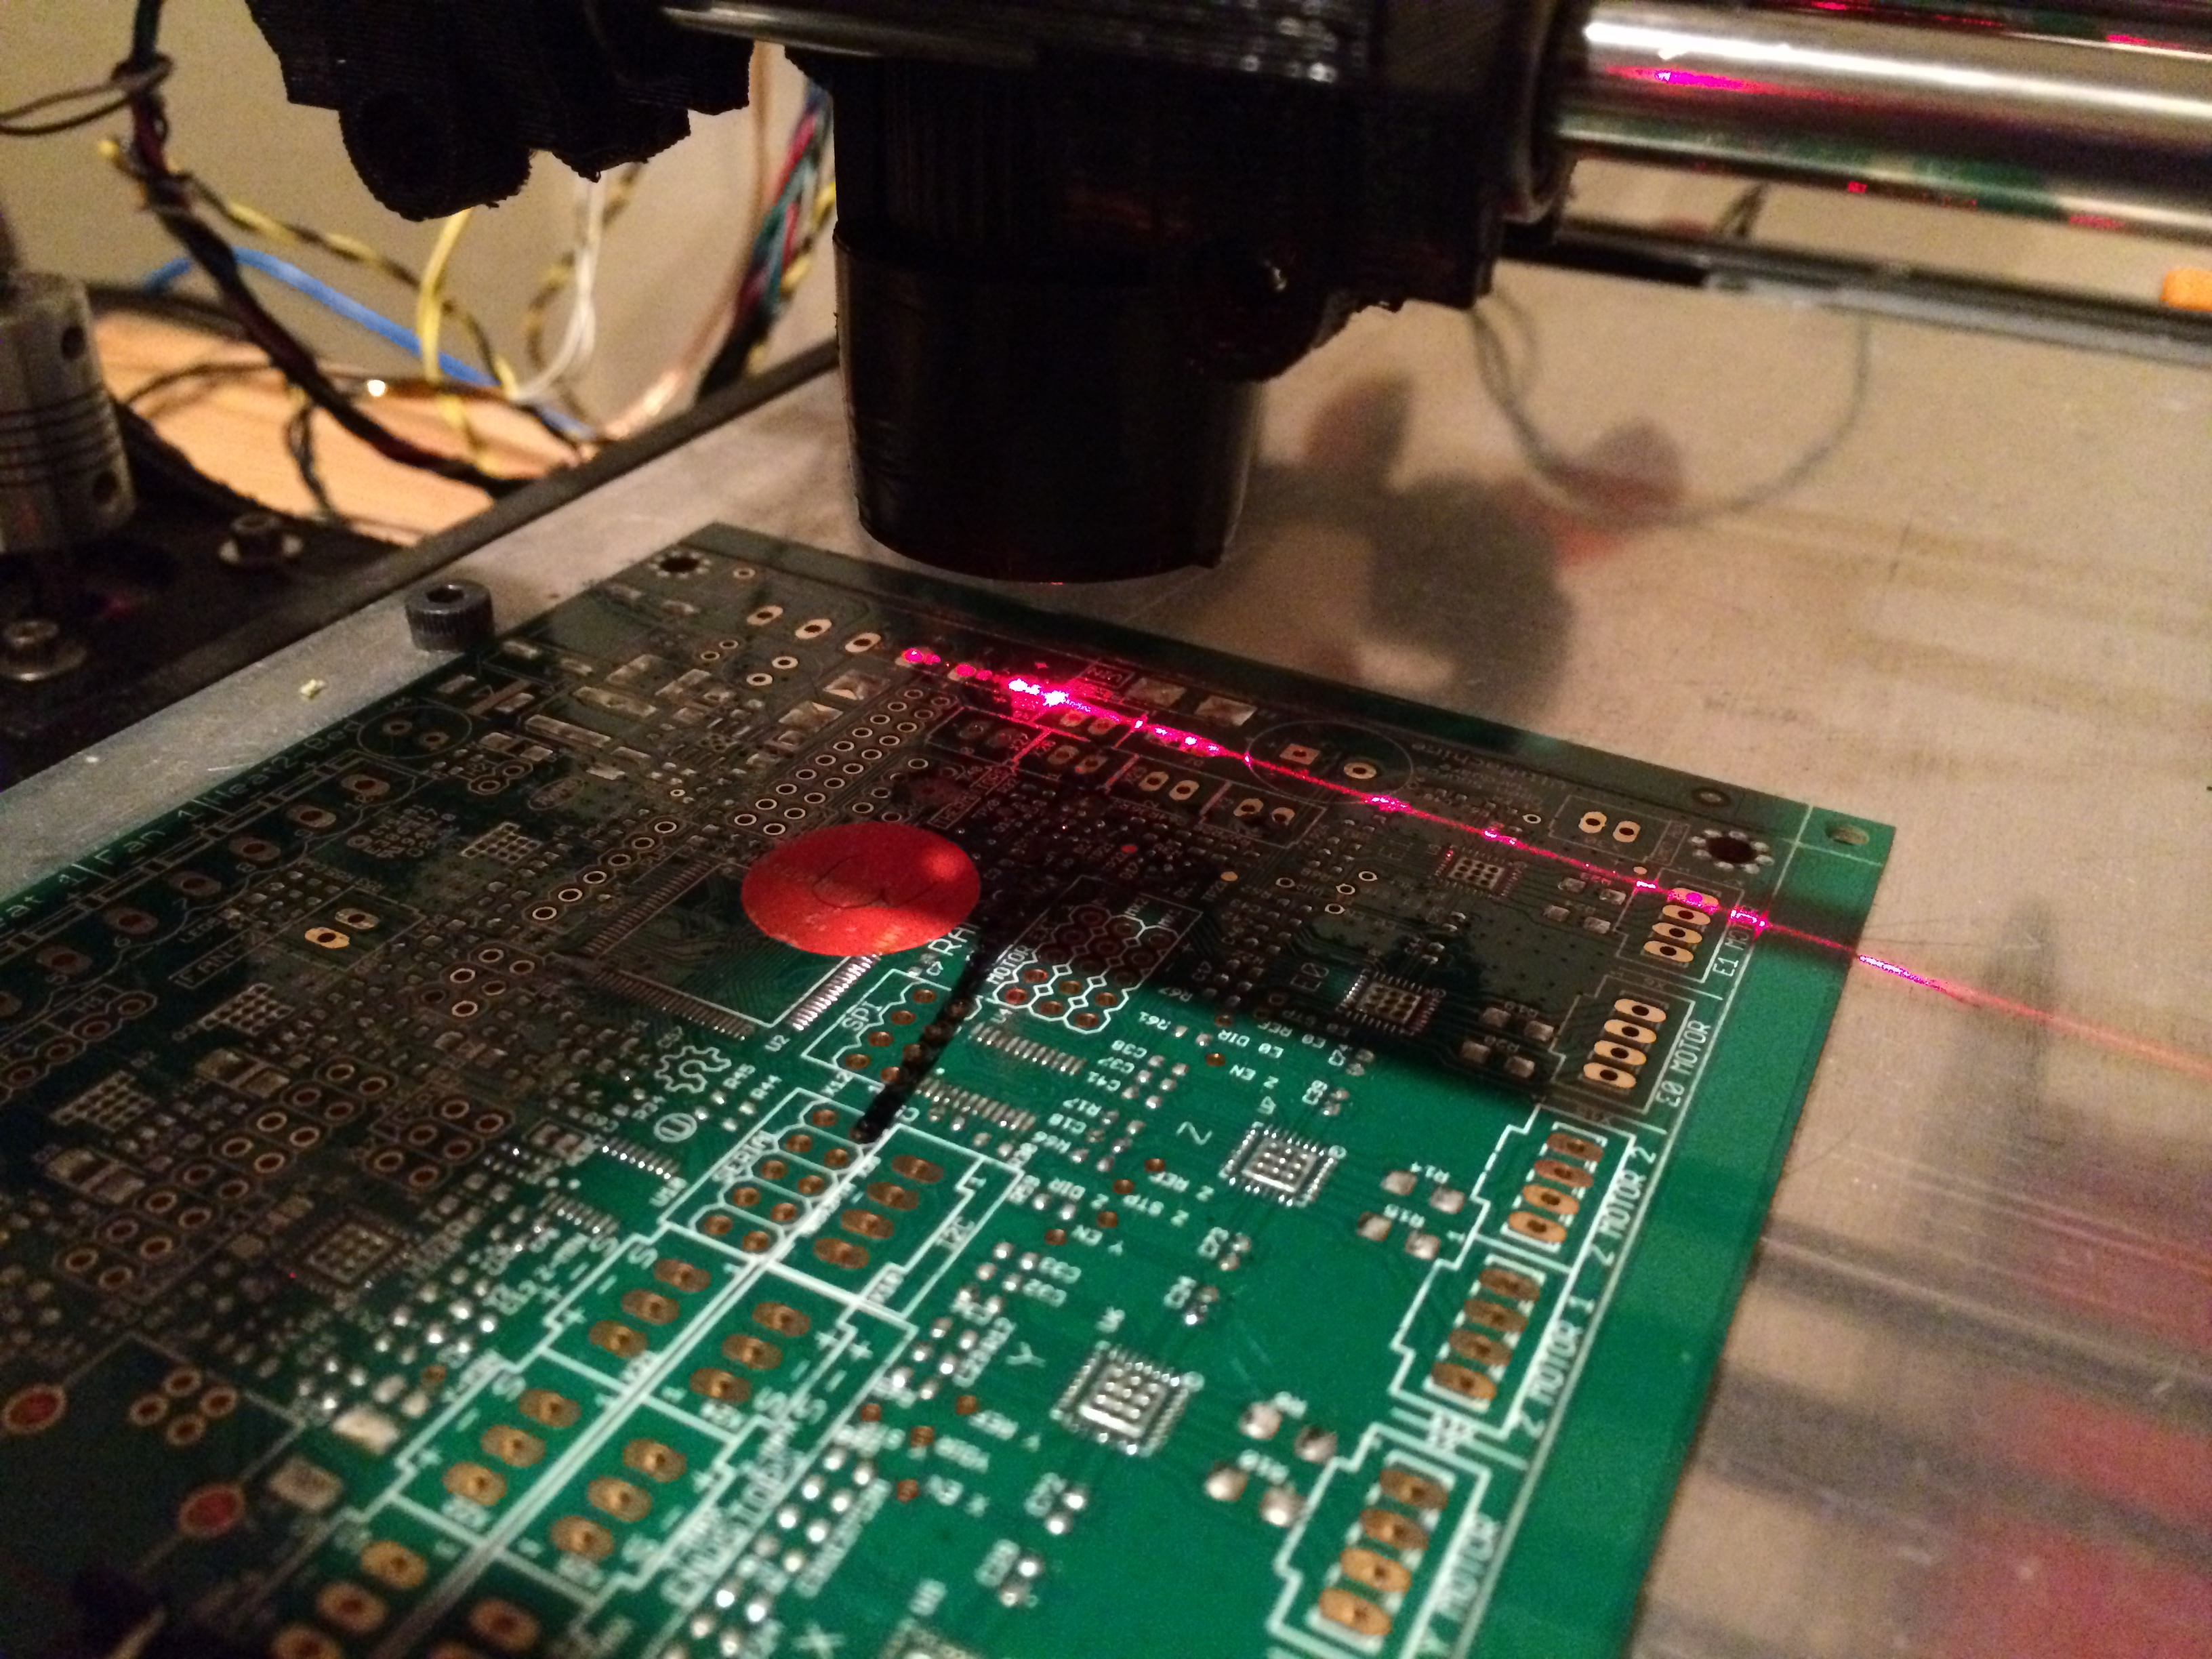
\includegraphics[scale=0.1,angle=270]{images/volume_analysis_setup/IMG_0606.JPG}
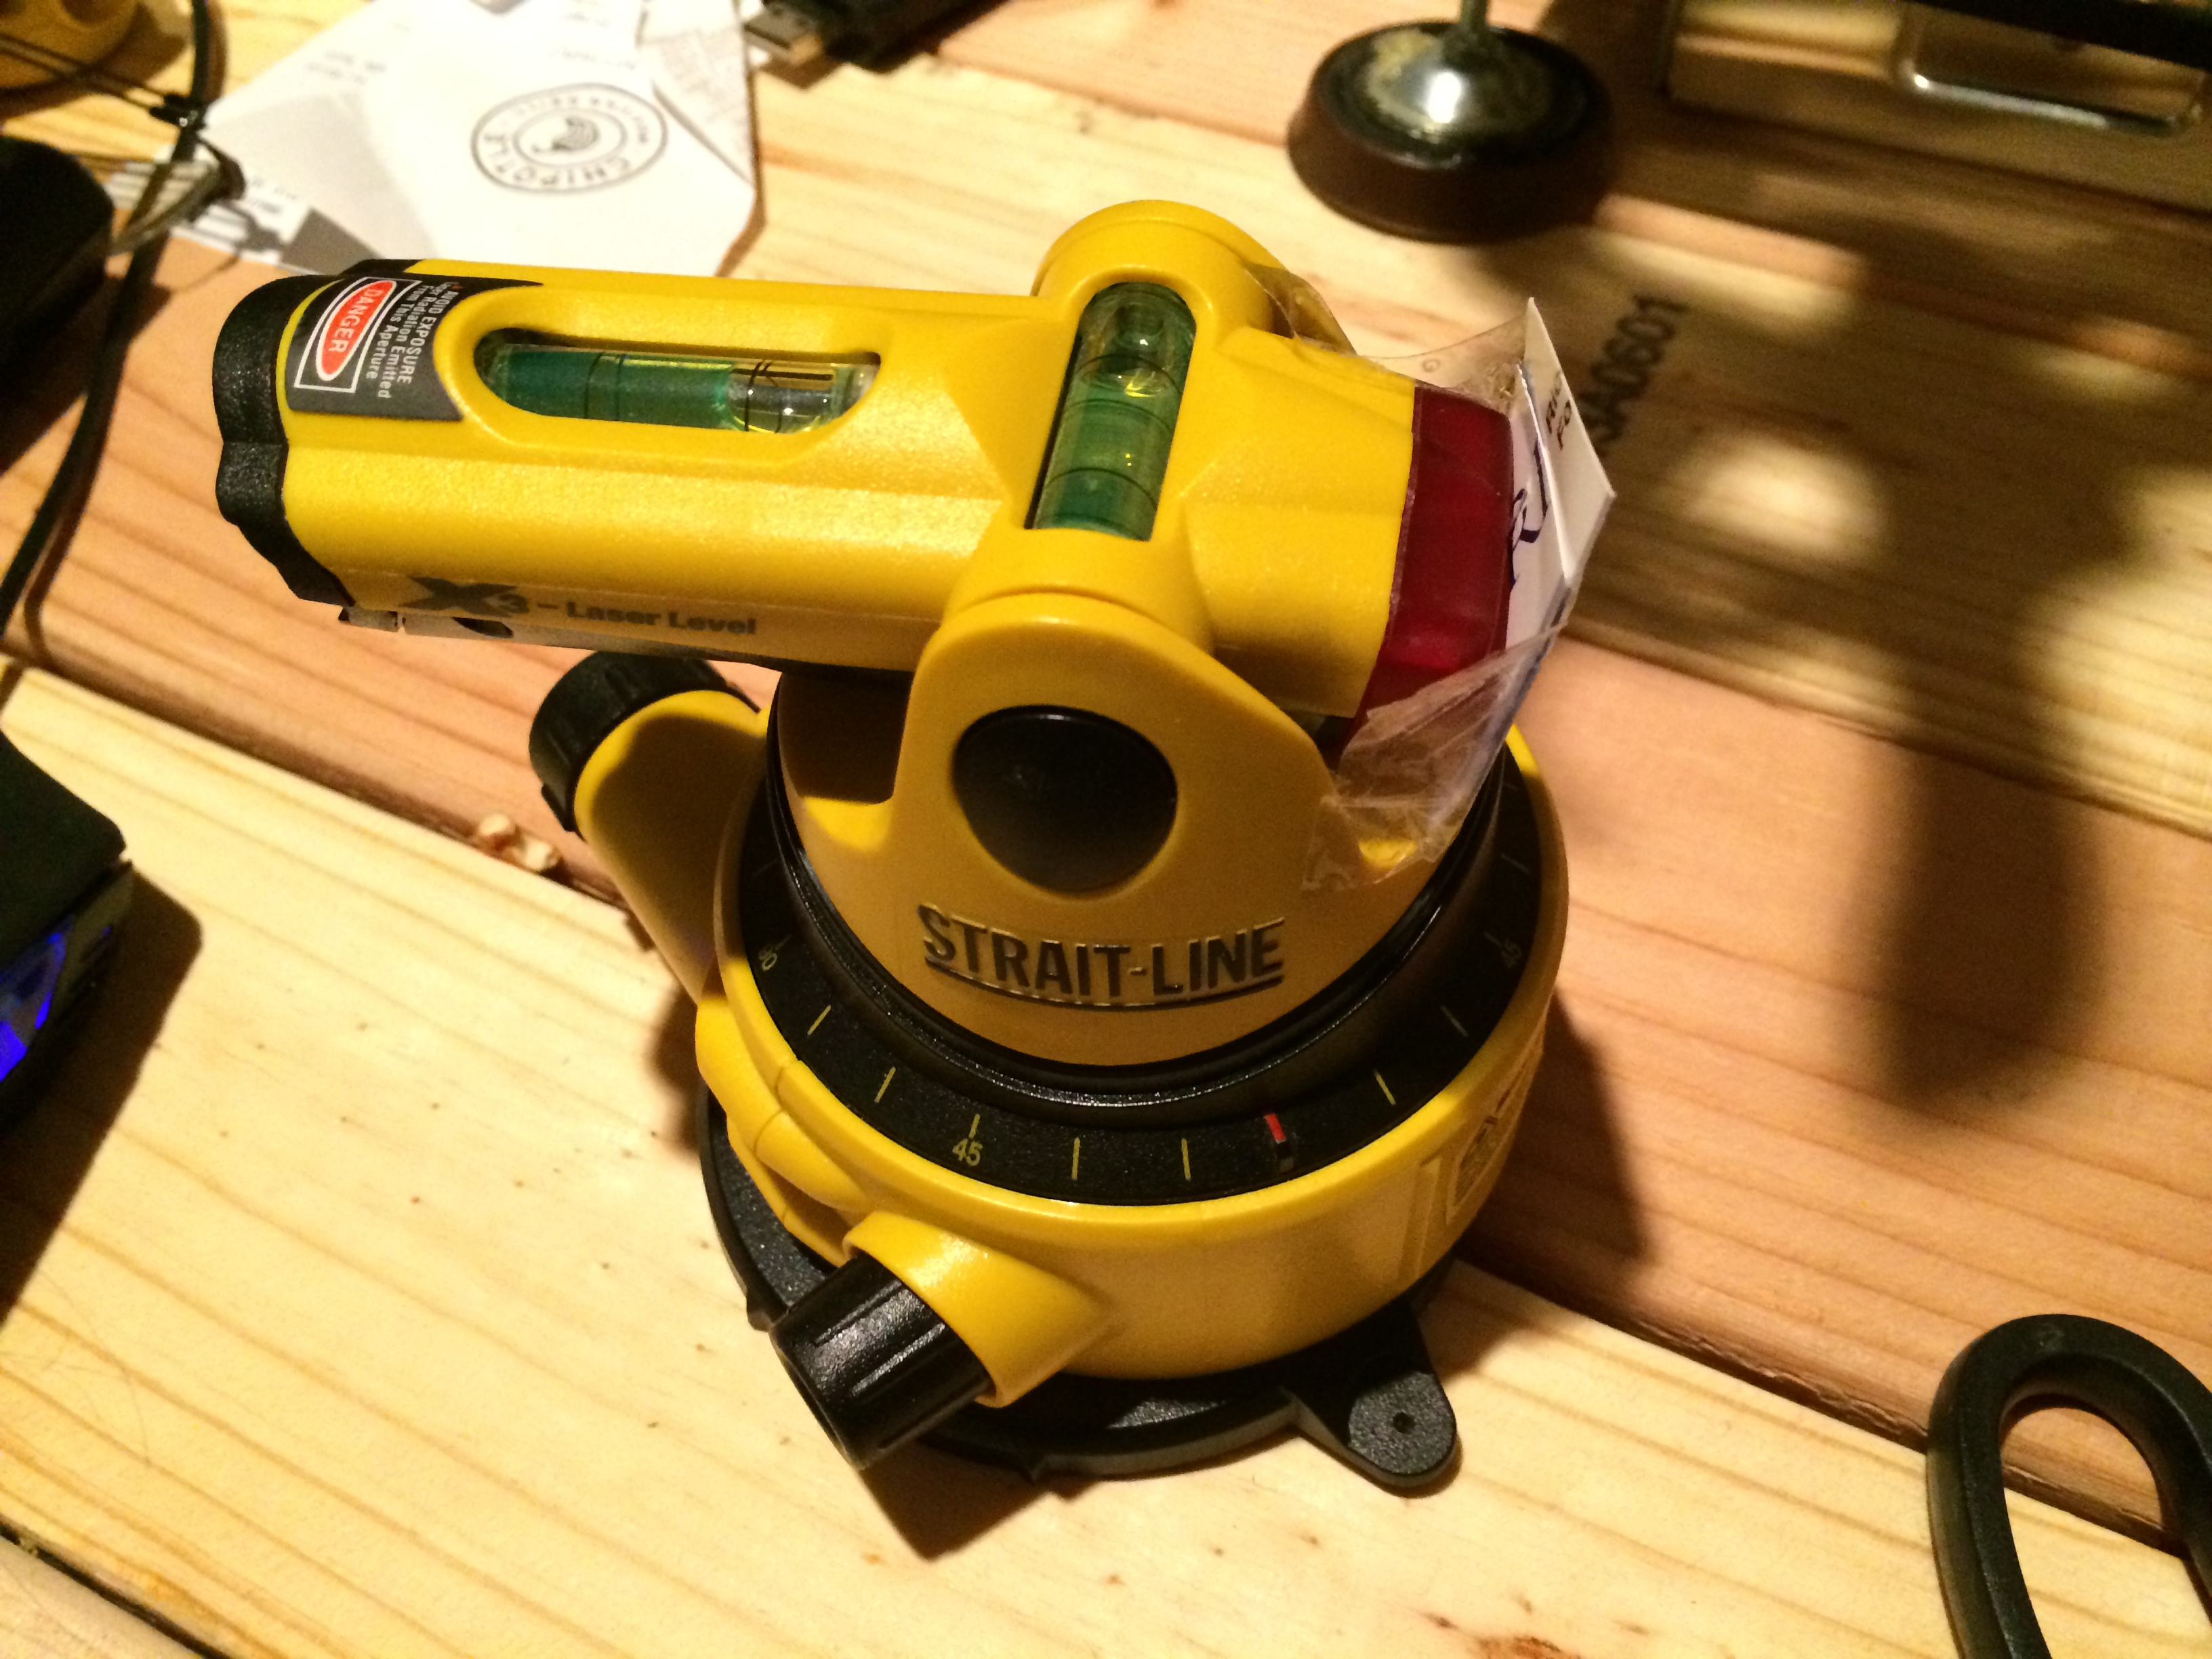
\includegraphics[scale=0.1,angle=270]{images/volume_analysis_setup/IMG_0607.JPG}
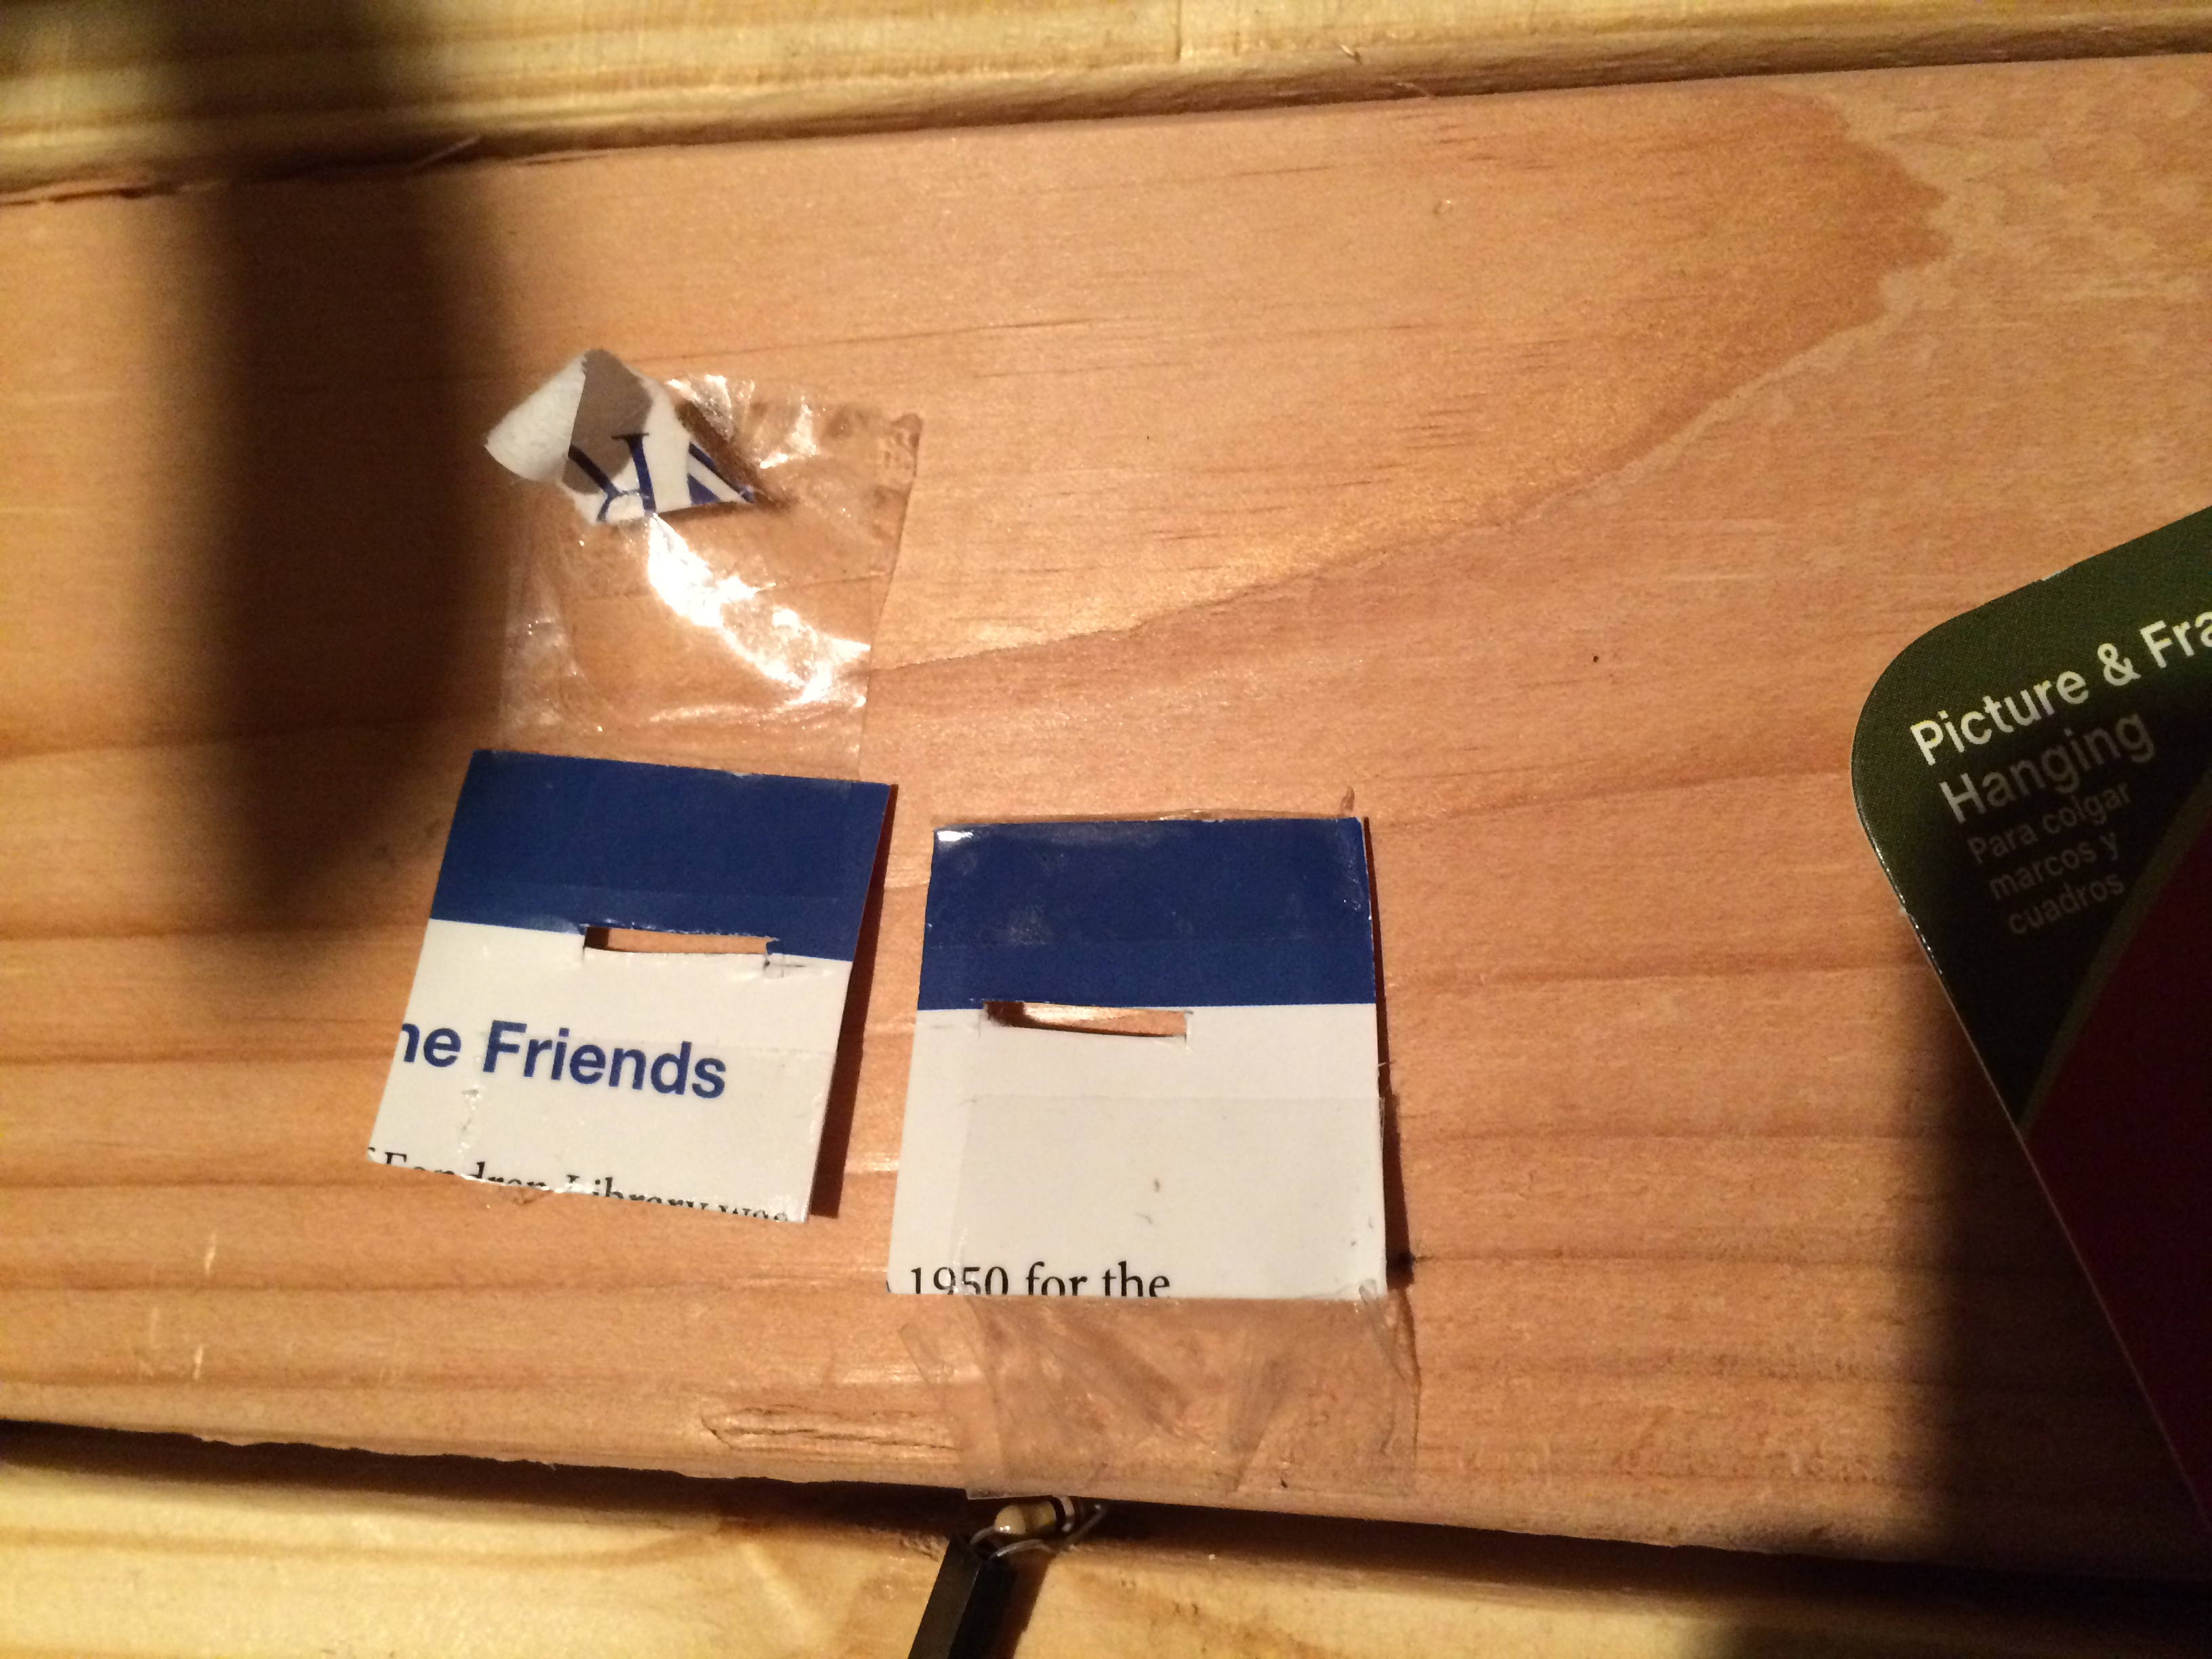
\includegraphics[scale=0.1,angle=270]{images/volume_analysis_setup/IMG_0608.JPG}
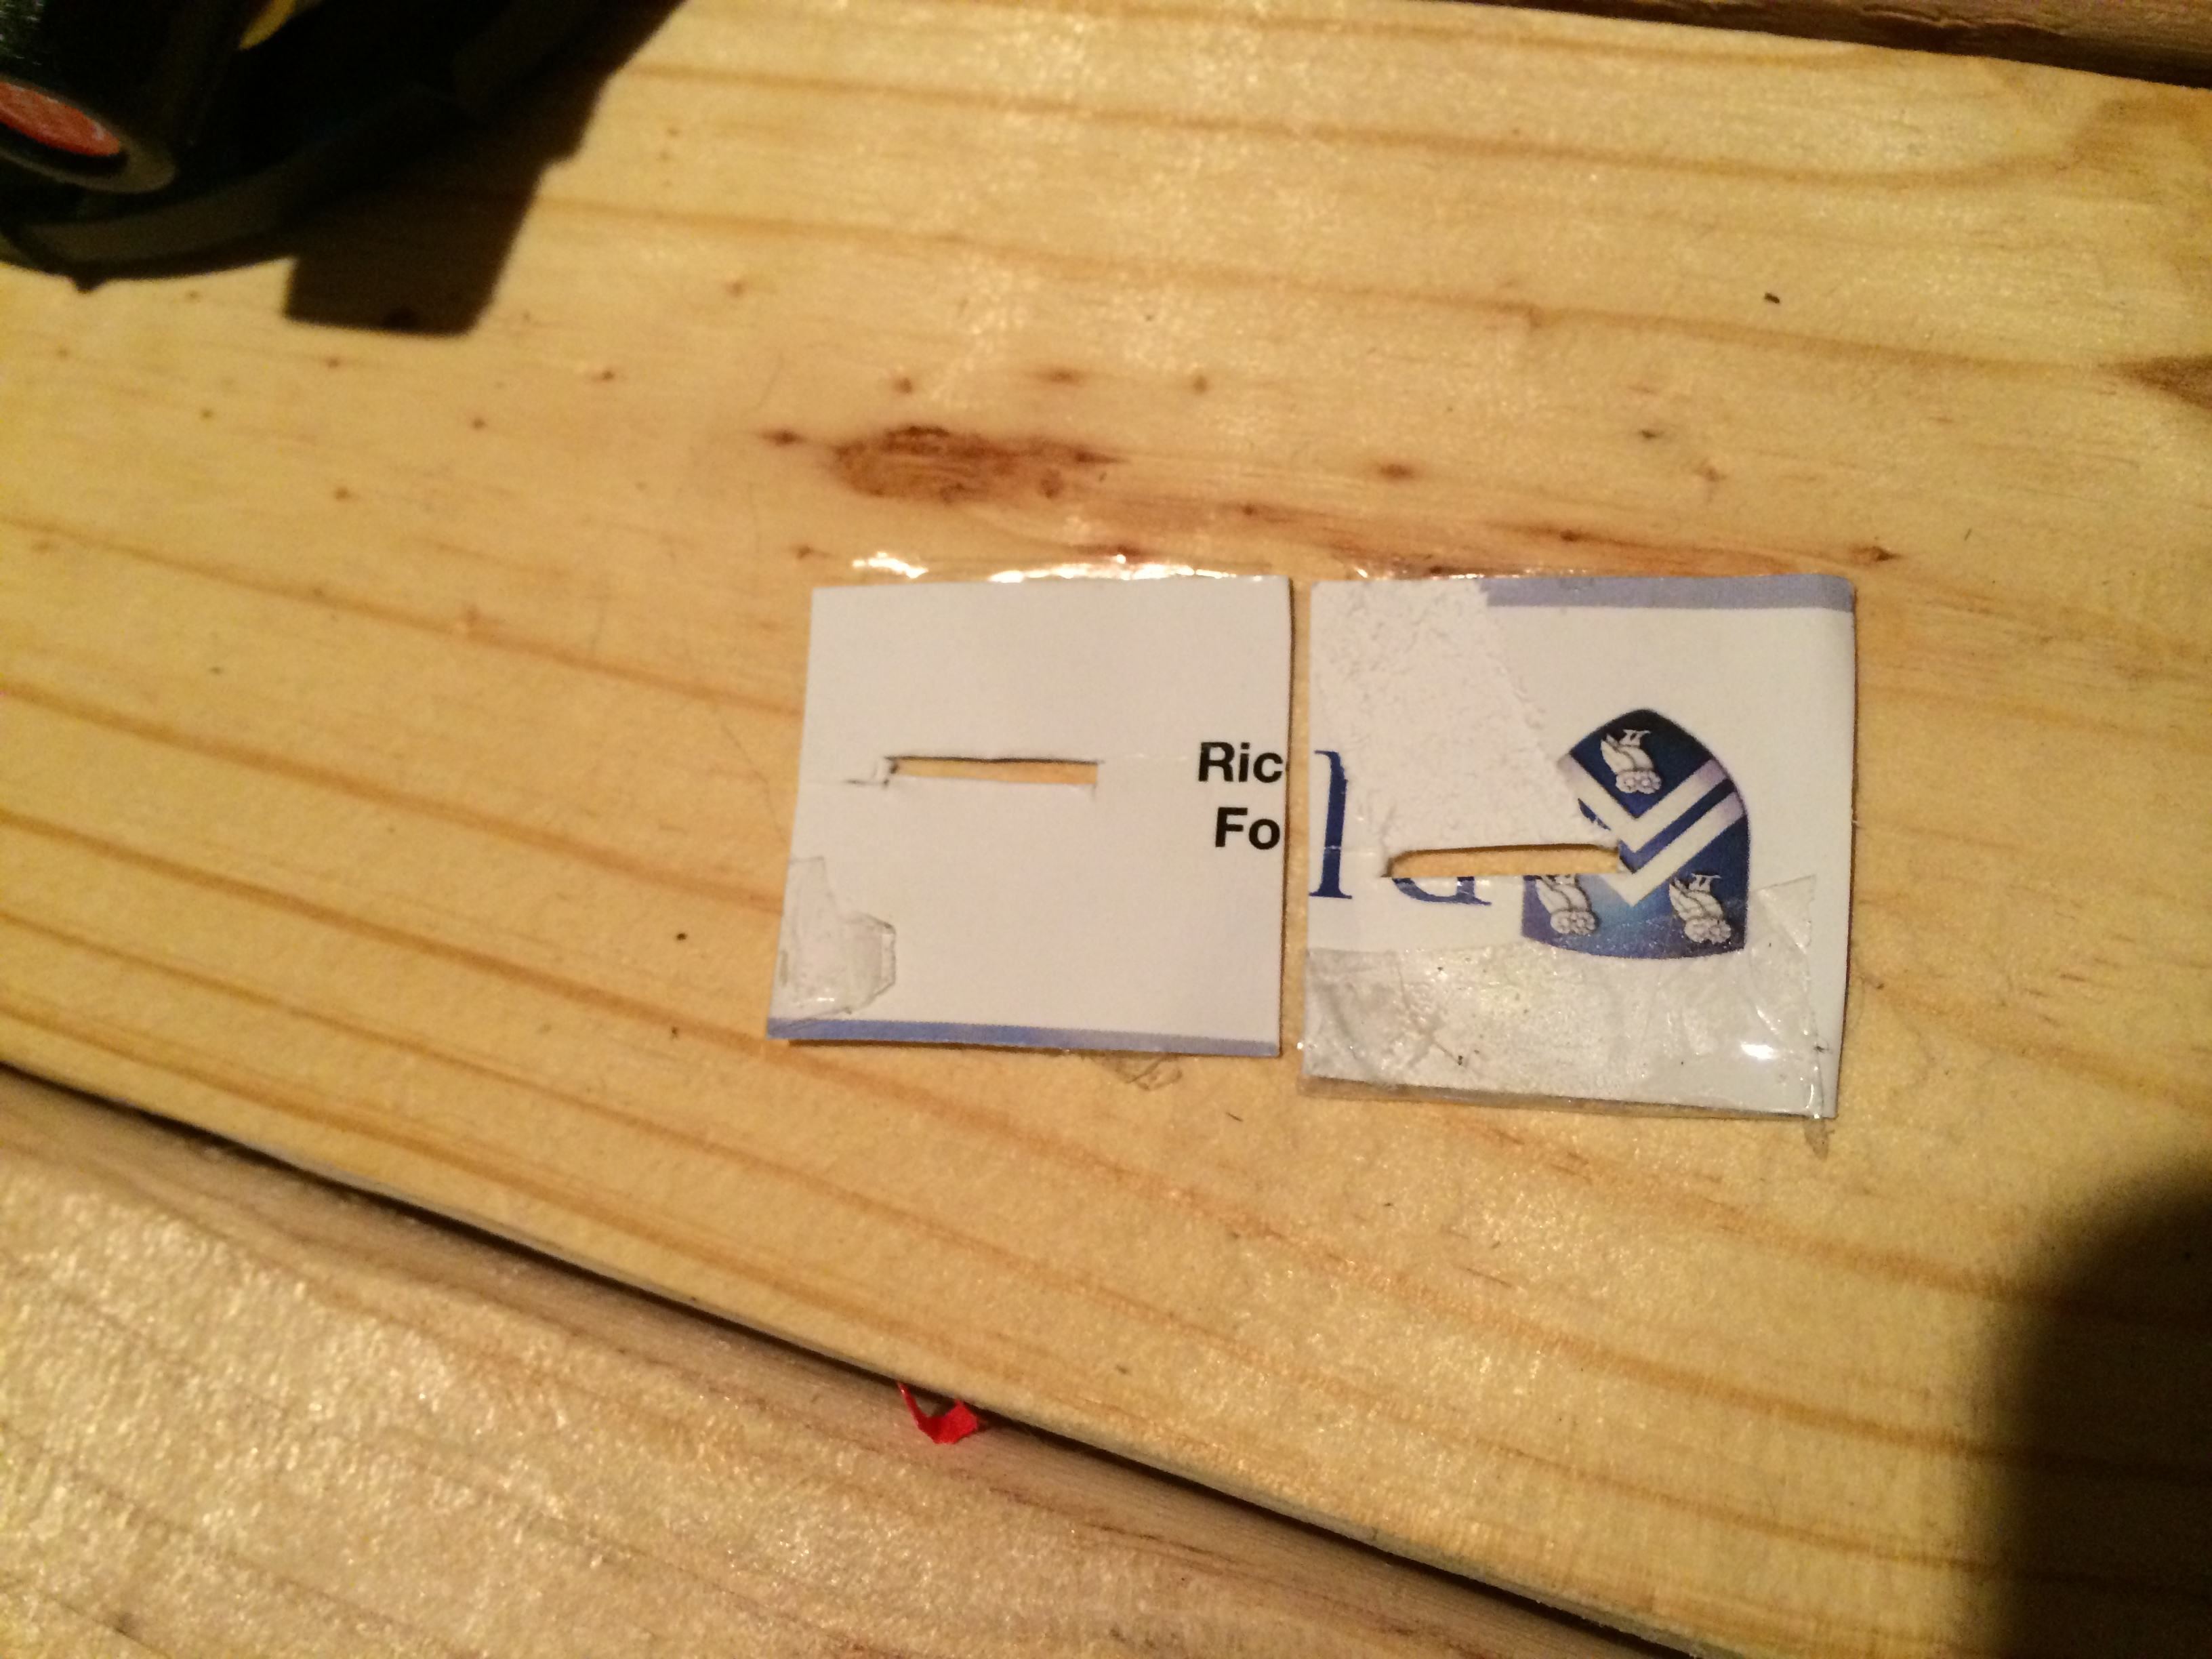
\includegraphics[scale=0.1,angle=270]{images/volume_analysis_setup/IMG_0609.JPG}
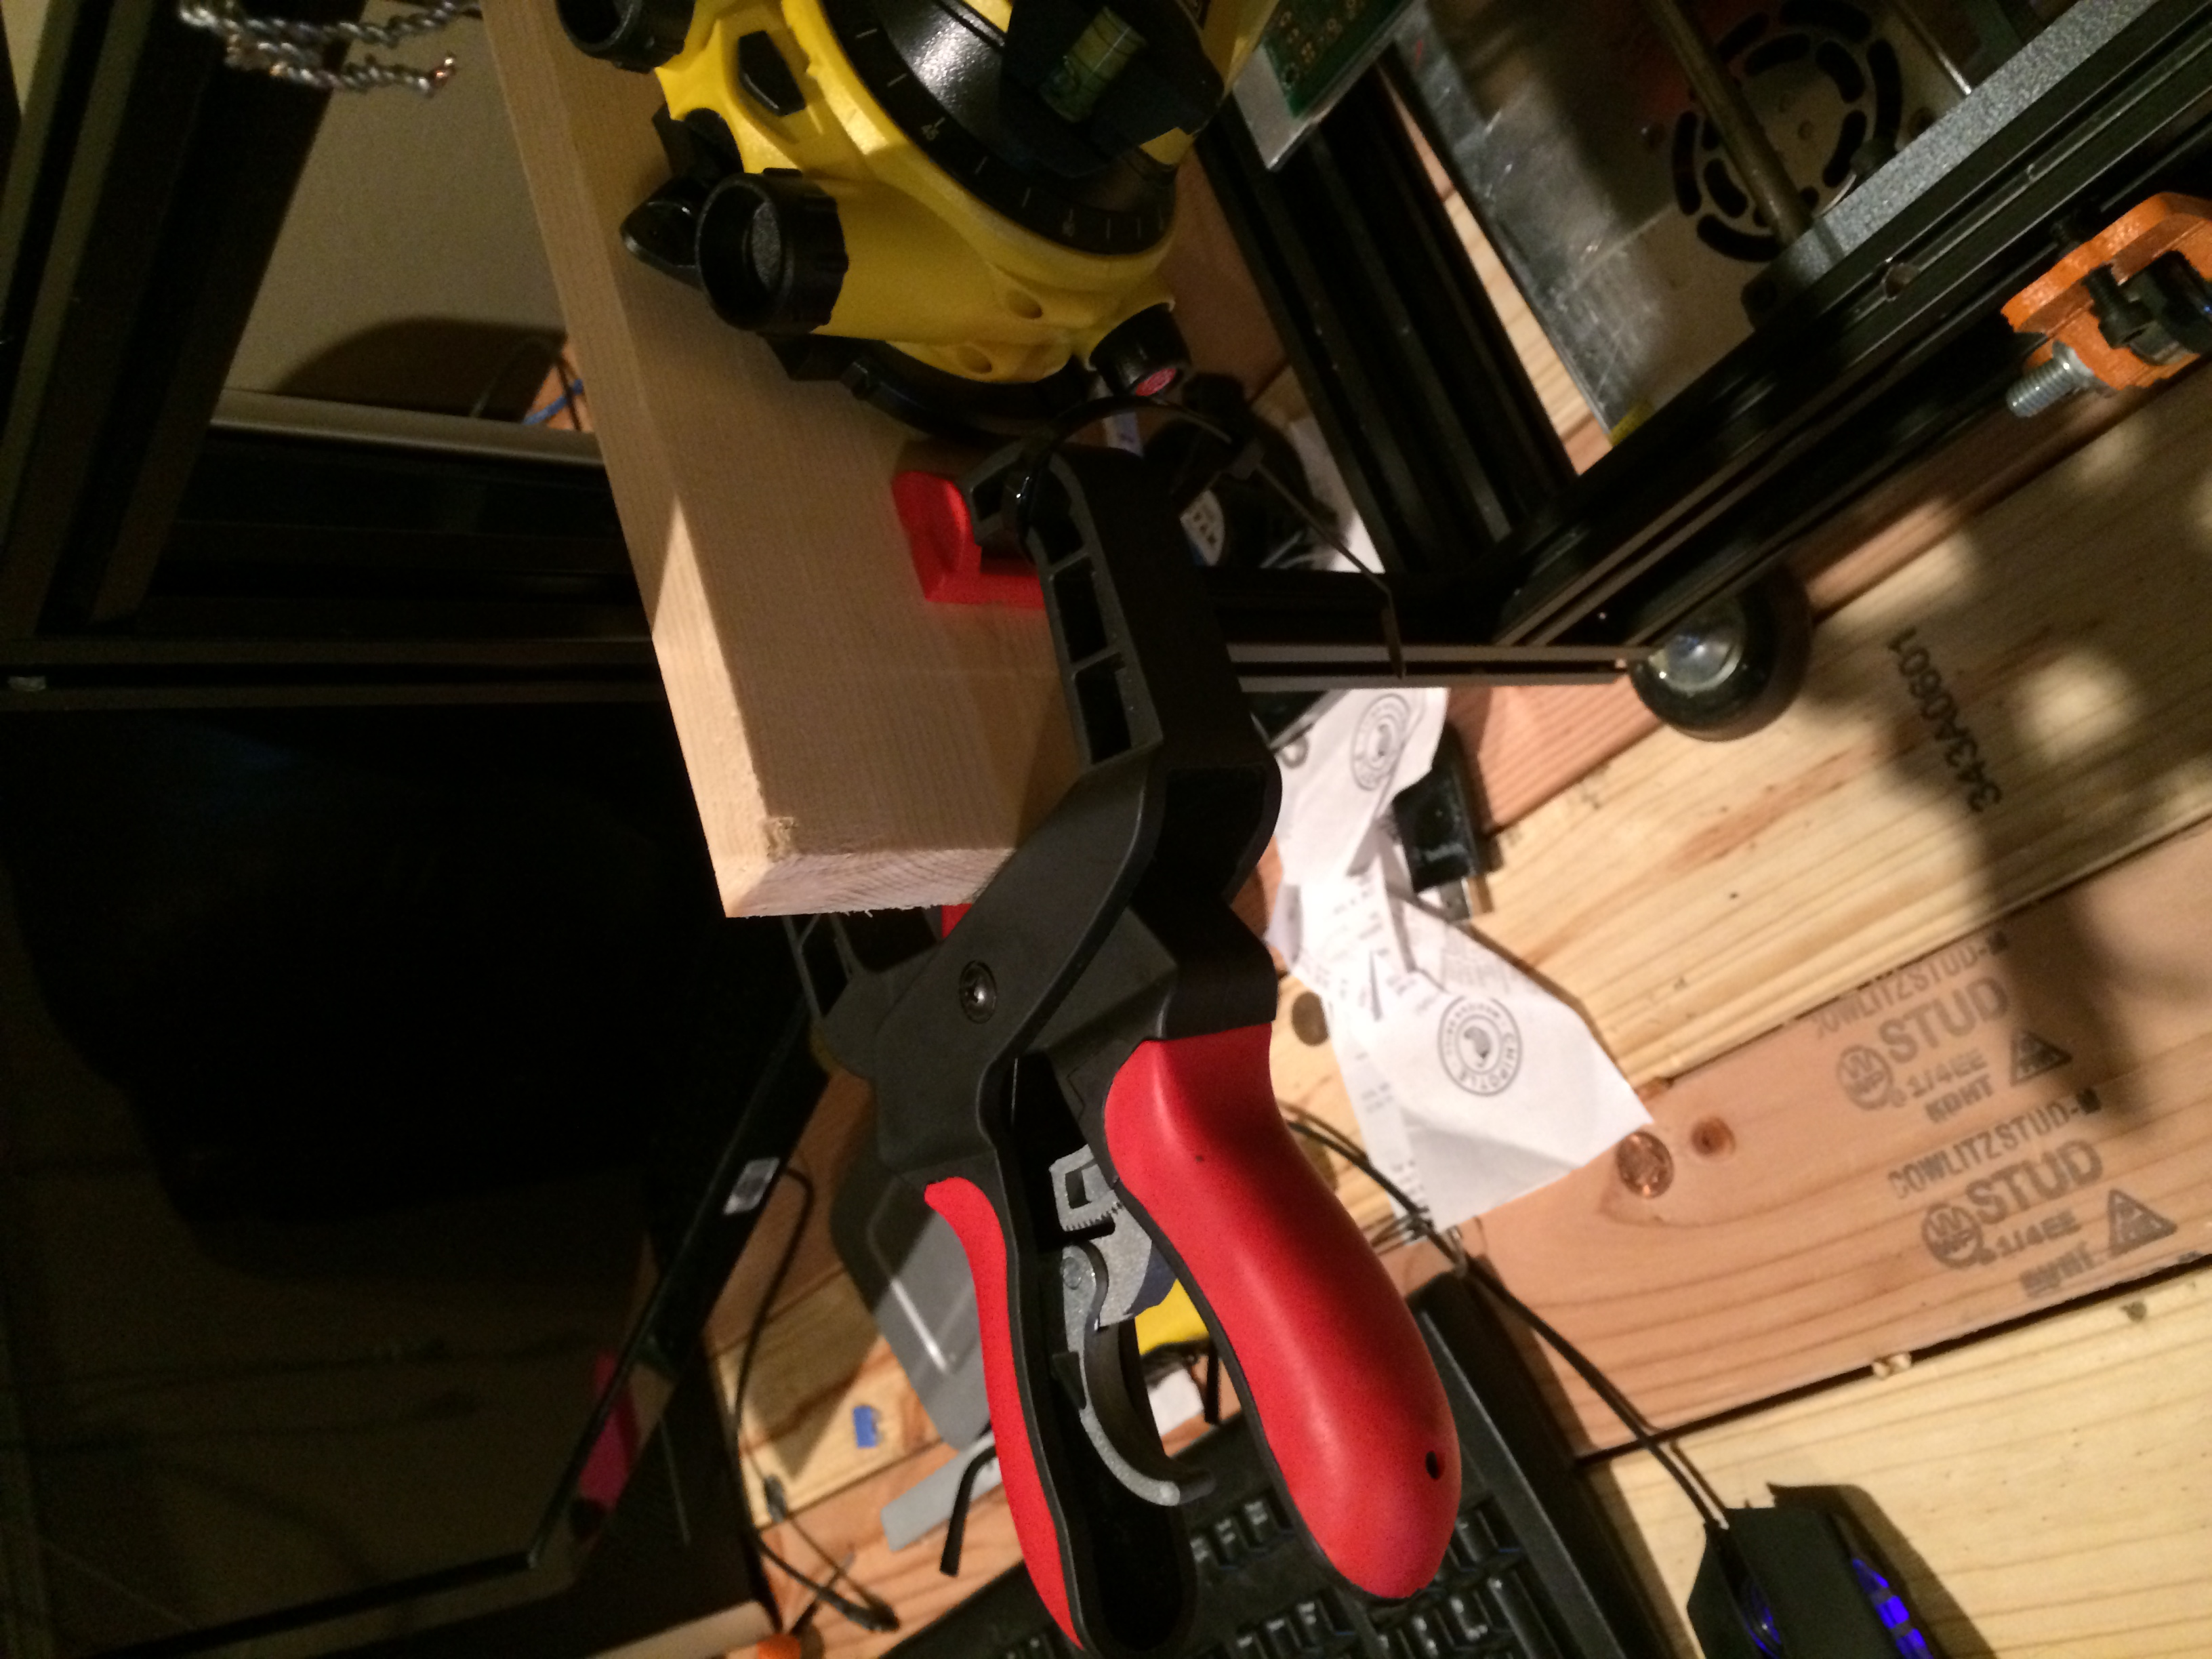
\includegraphics[scale=0.1,angle=270]{images/volume_analysis_setup/IMG_0610.JPG}
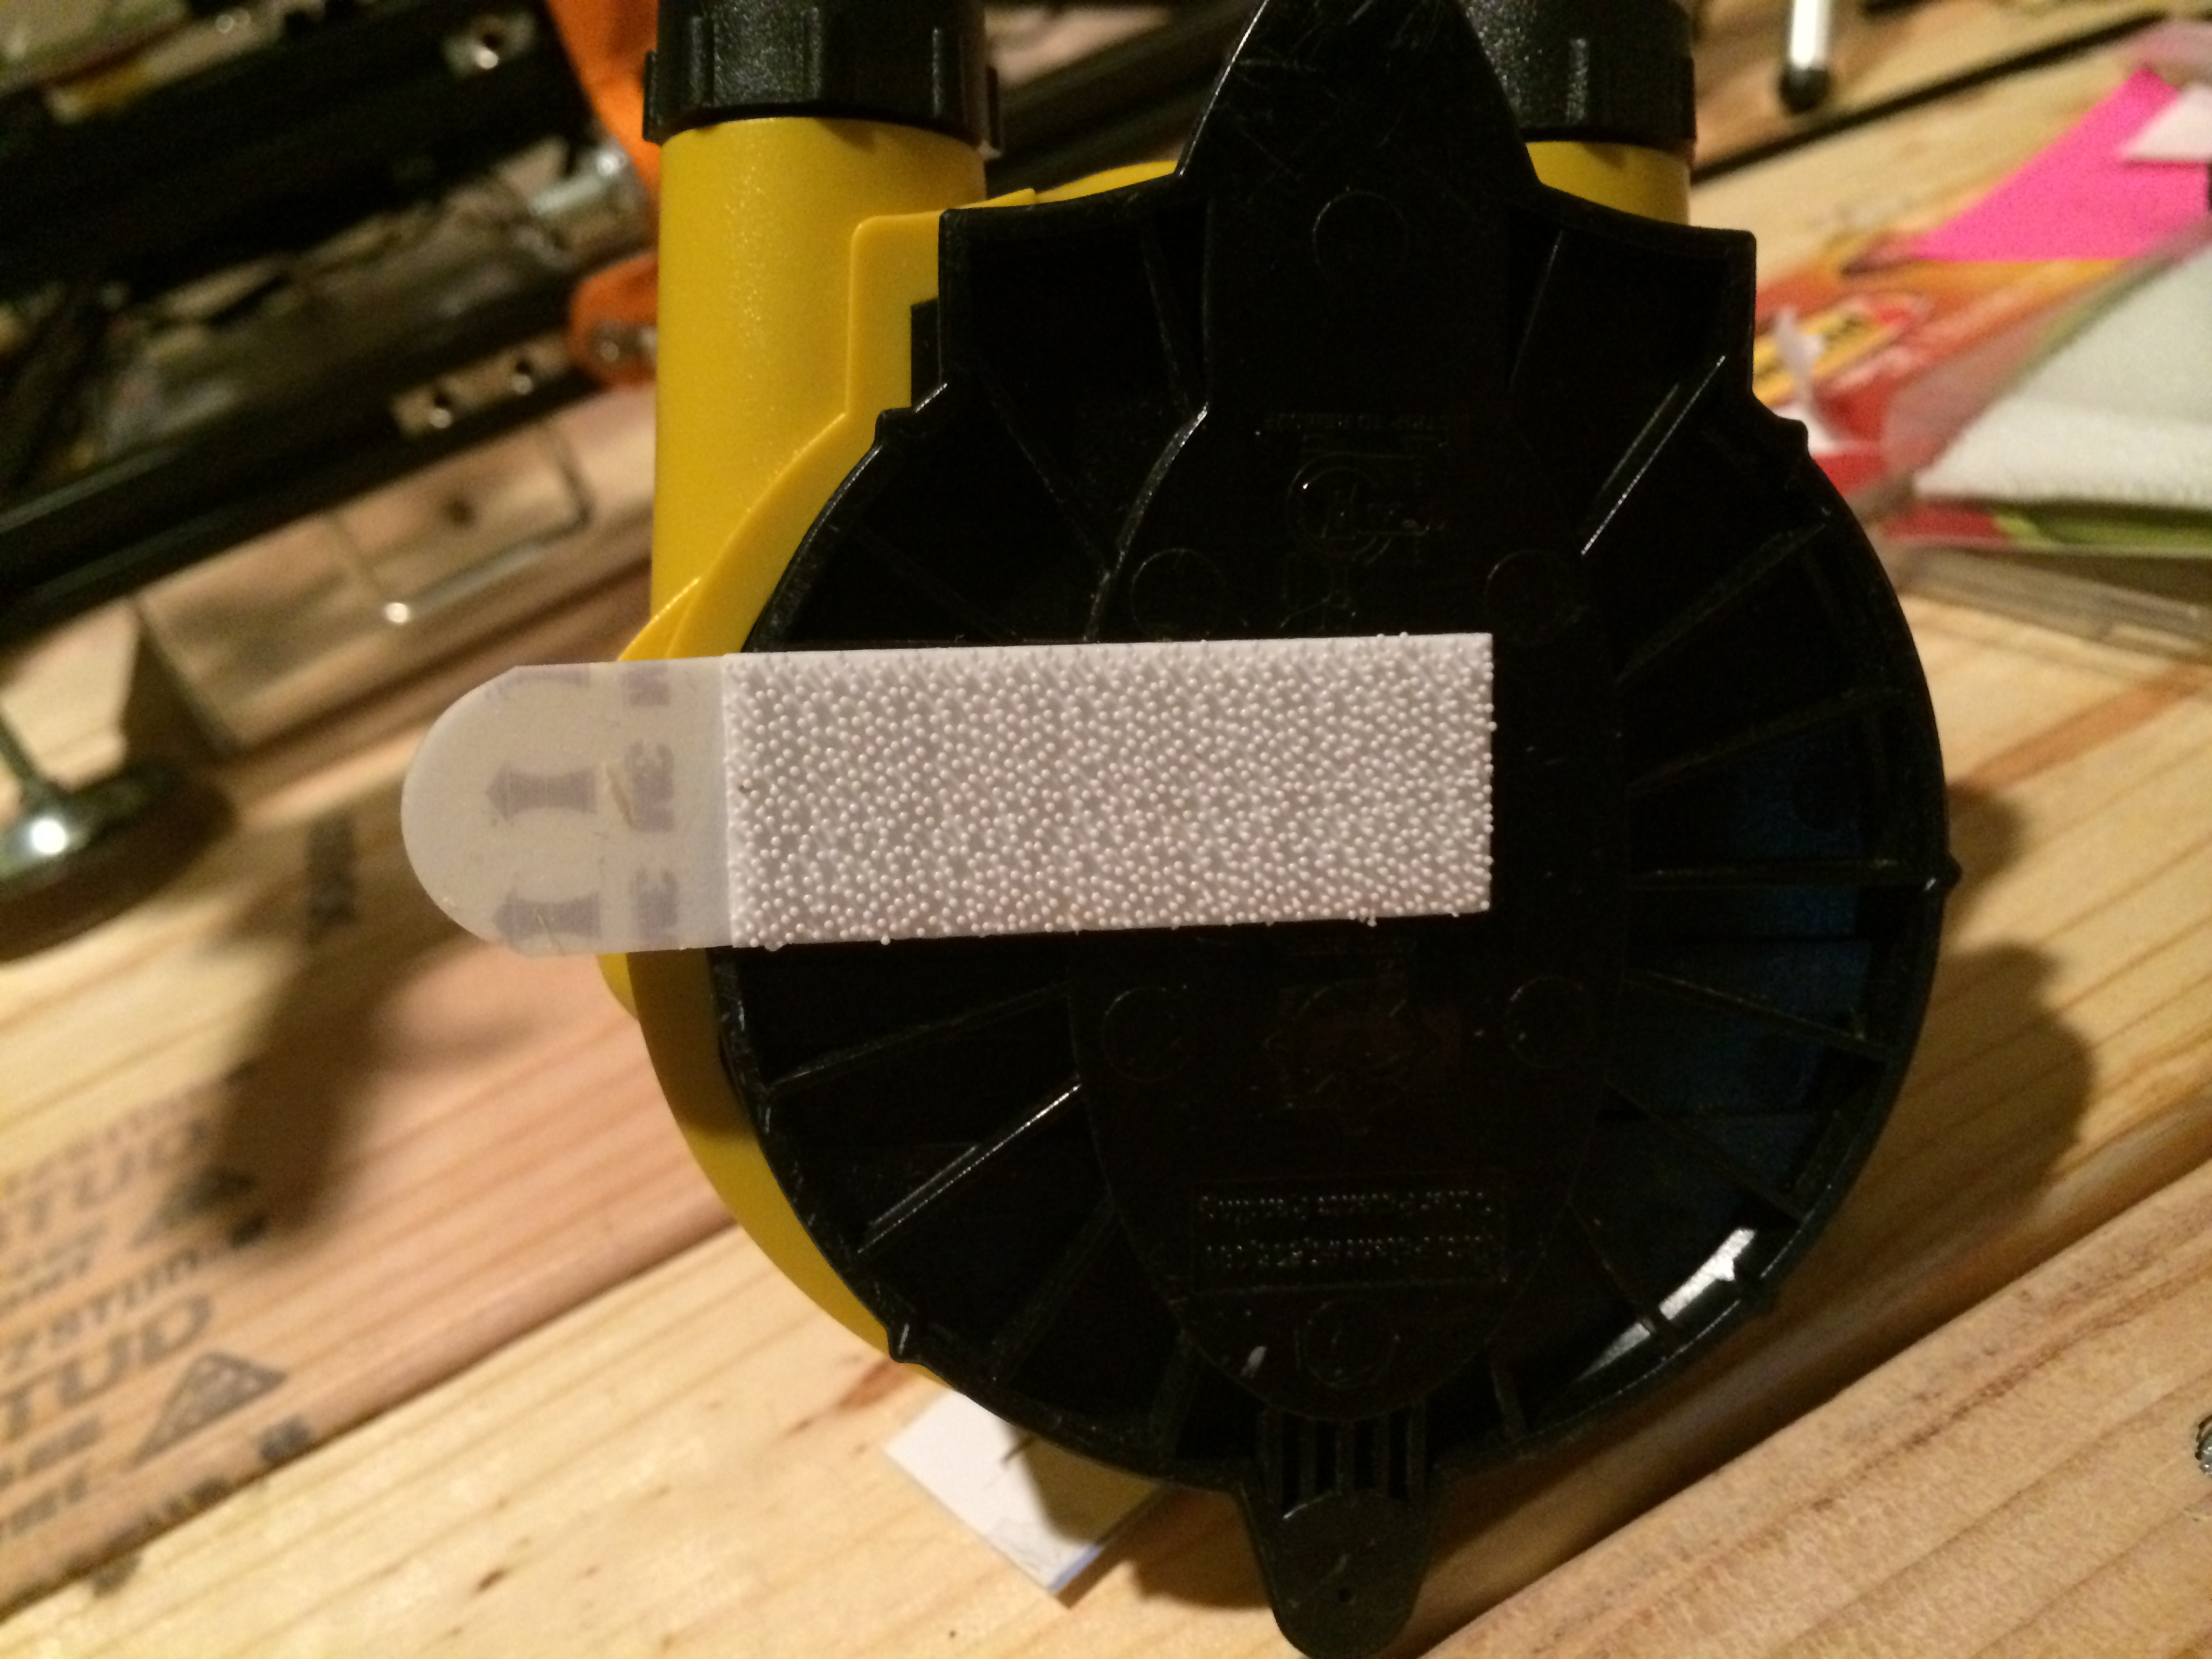
\includegraphics[scale=0.1,angle=270]{images/volume_analysis_setup/IMG_0611.JPG}
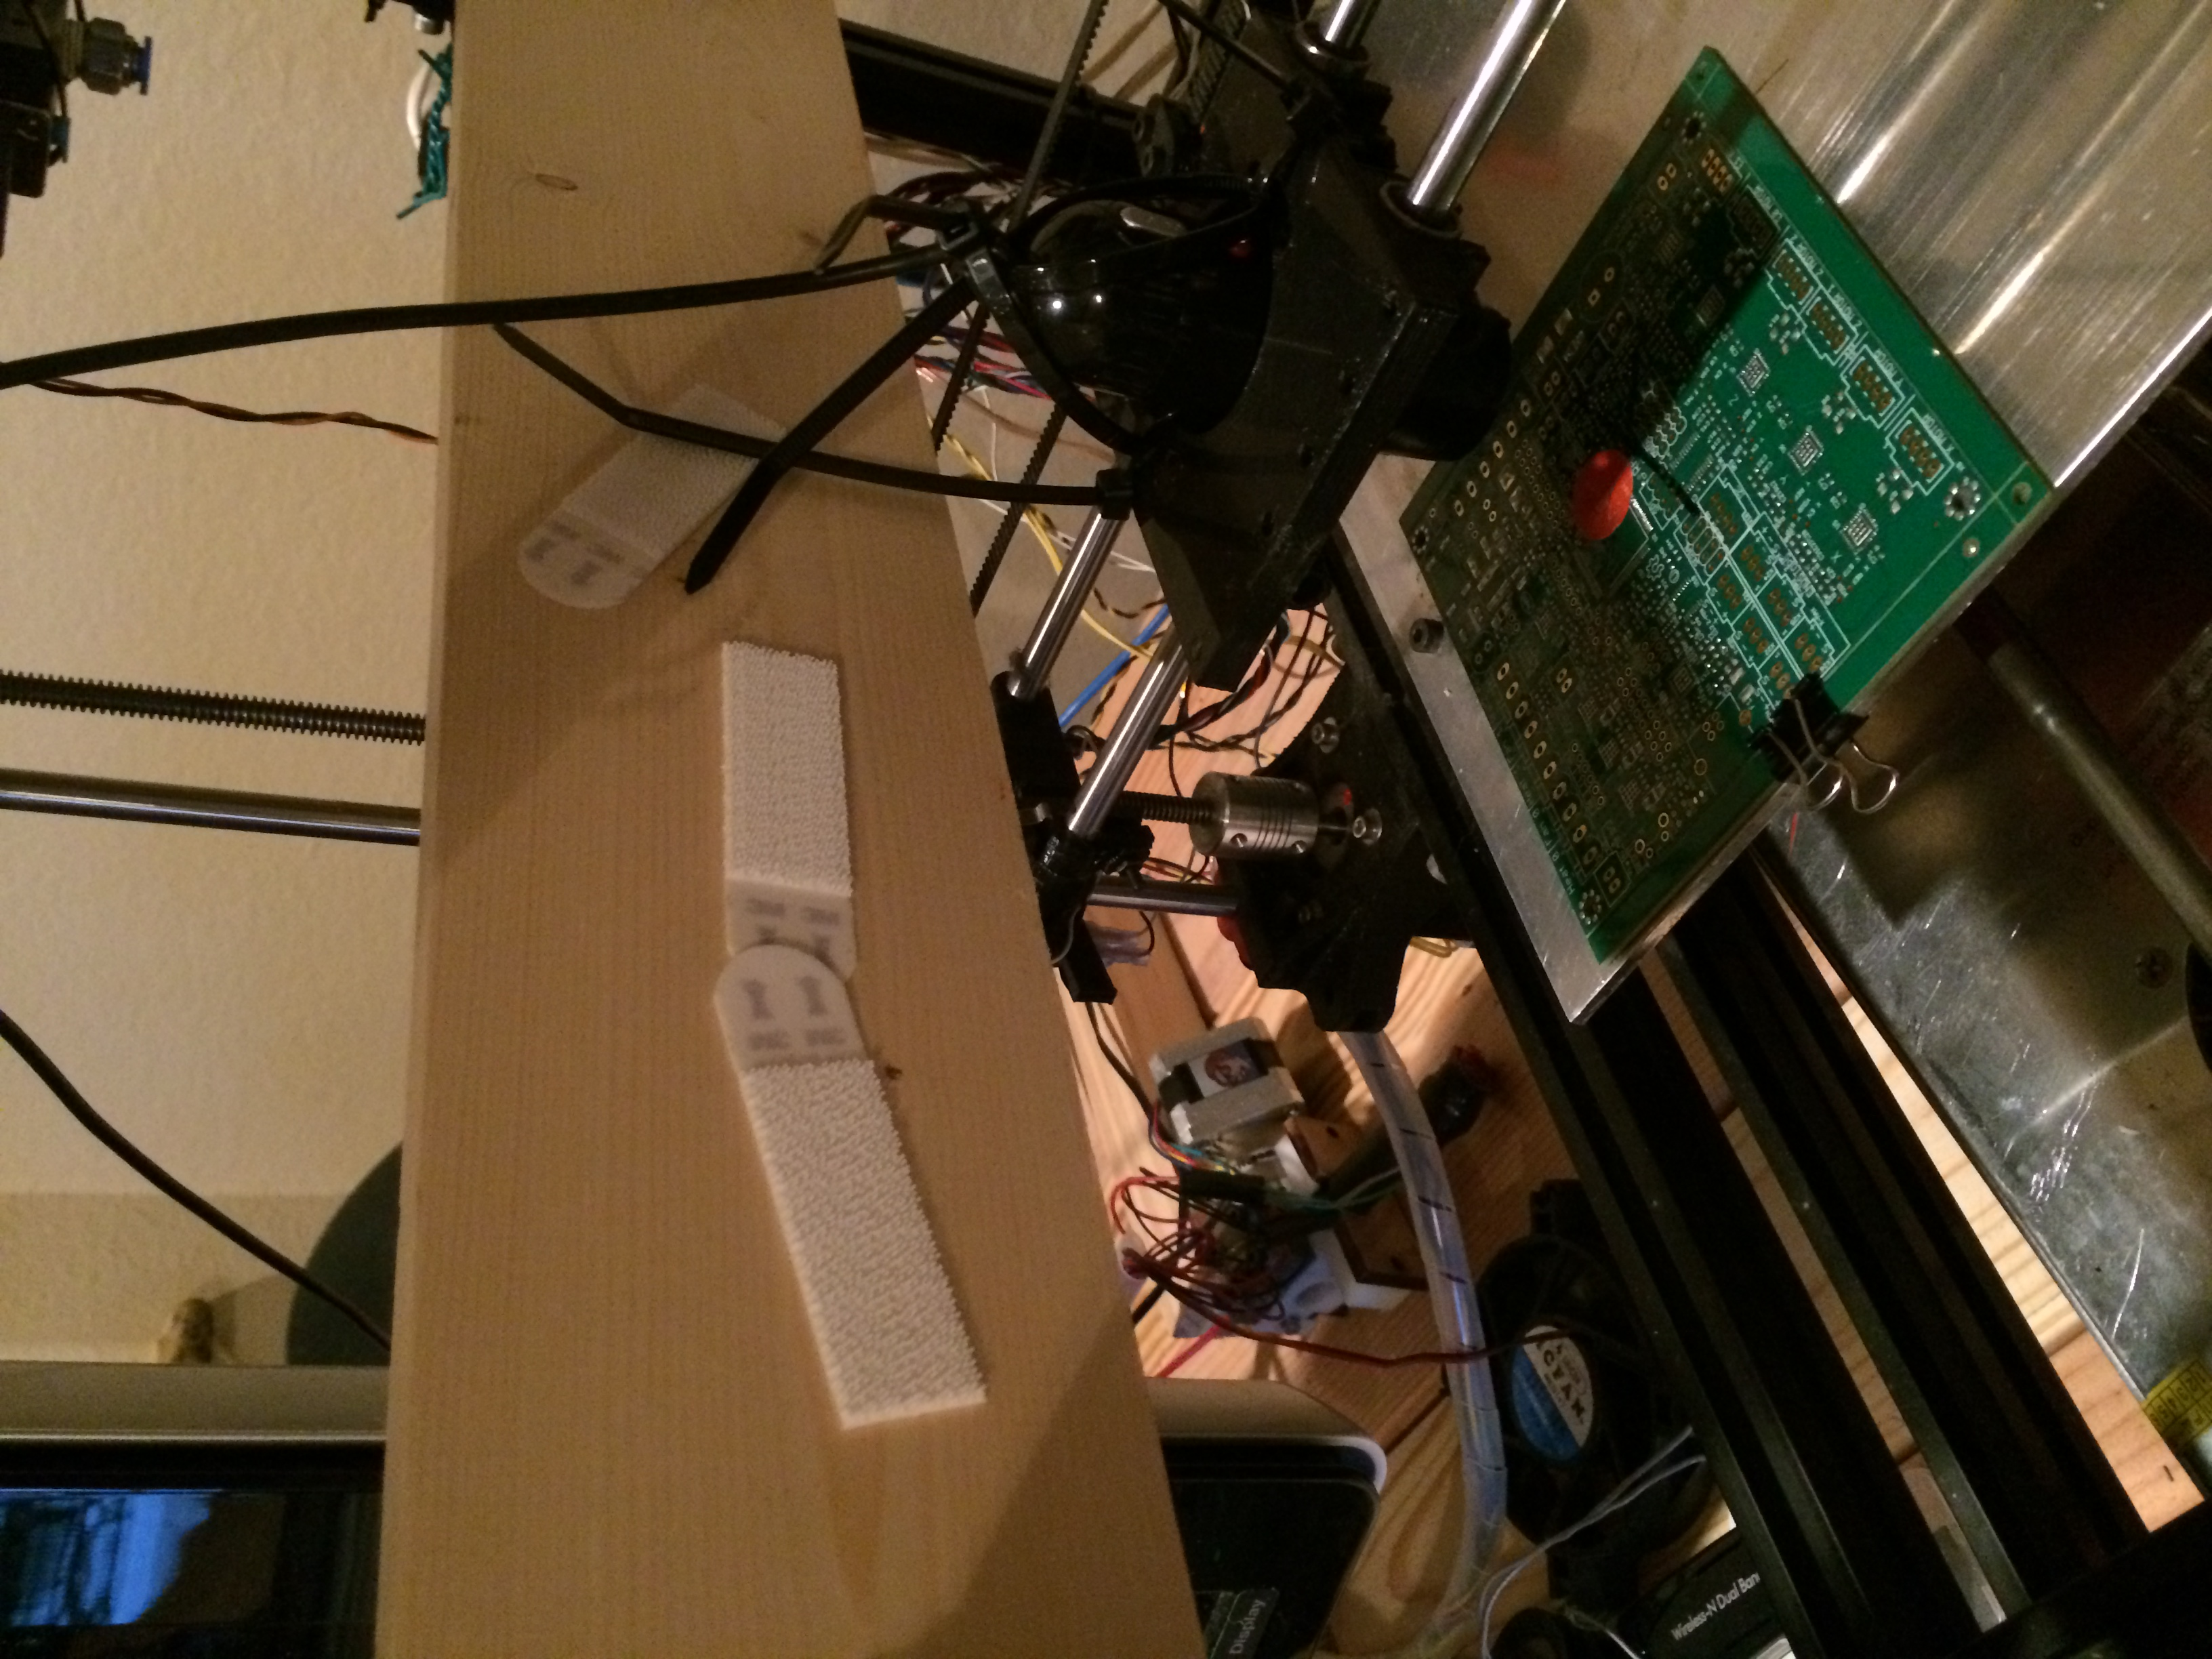
\includegraphics[scale=0.1,angle=270]{images/volume_analysis_setup/IMG_0612.JPG}
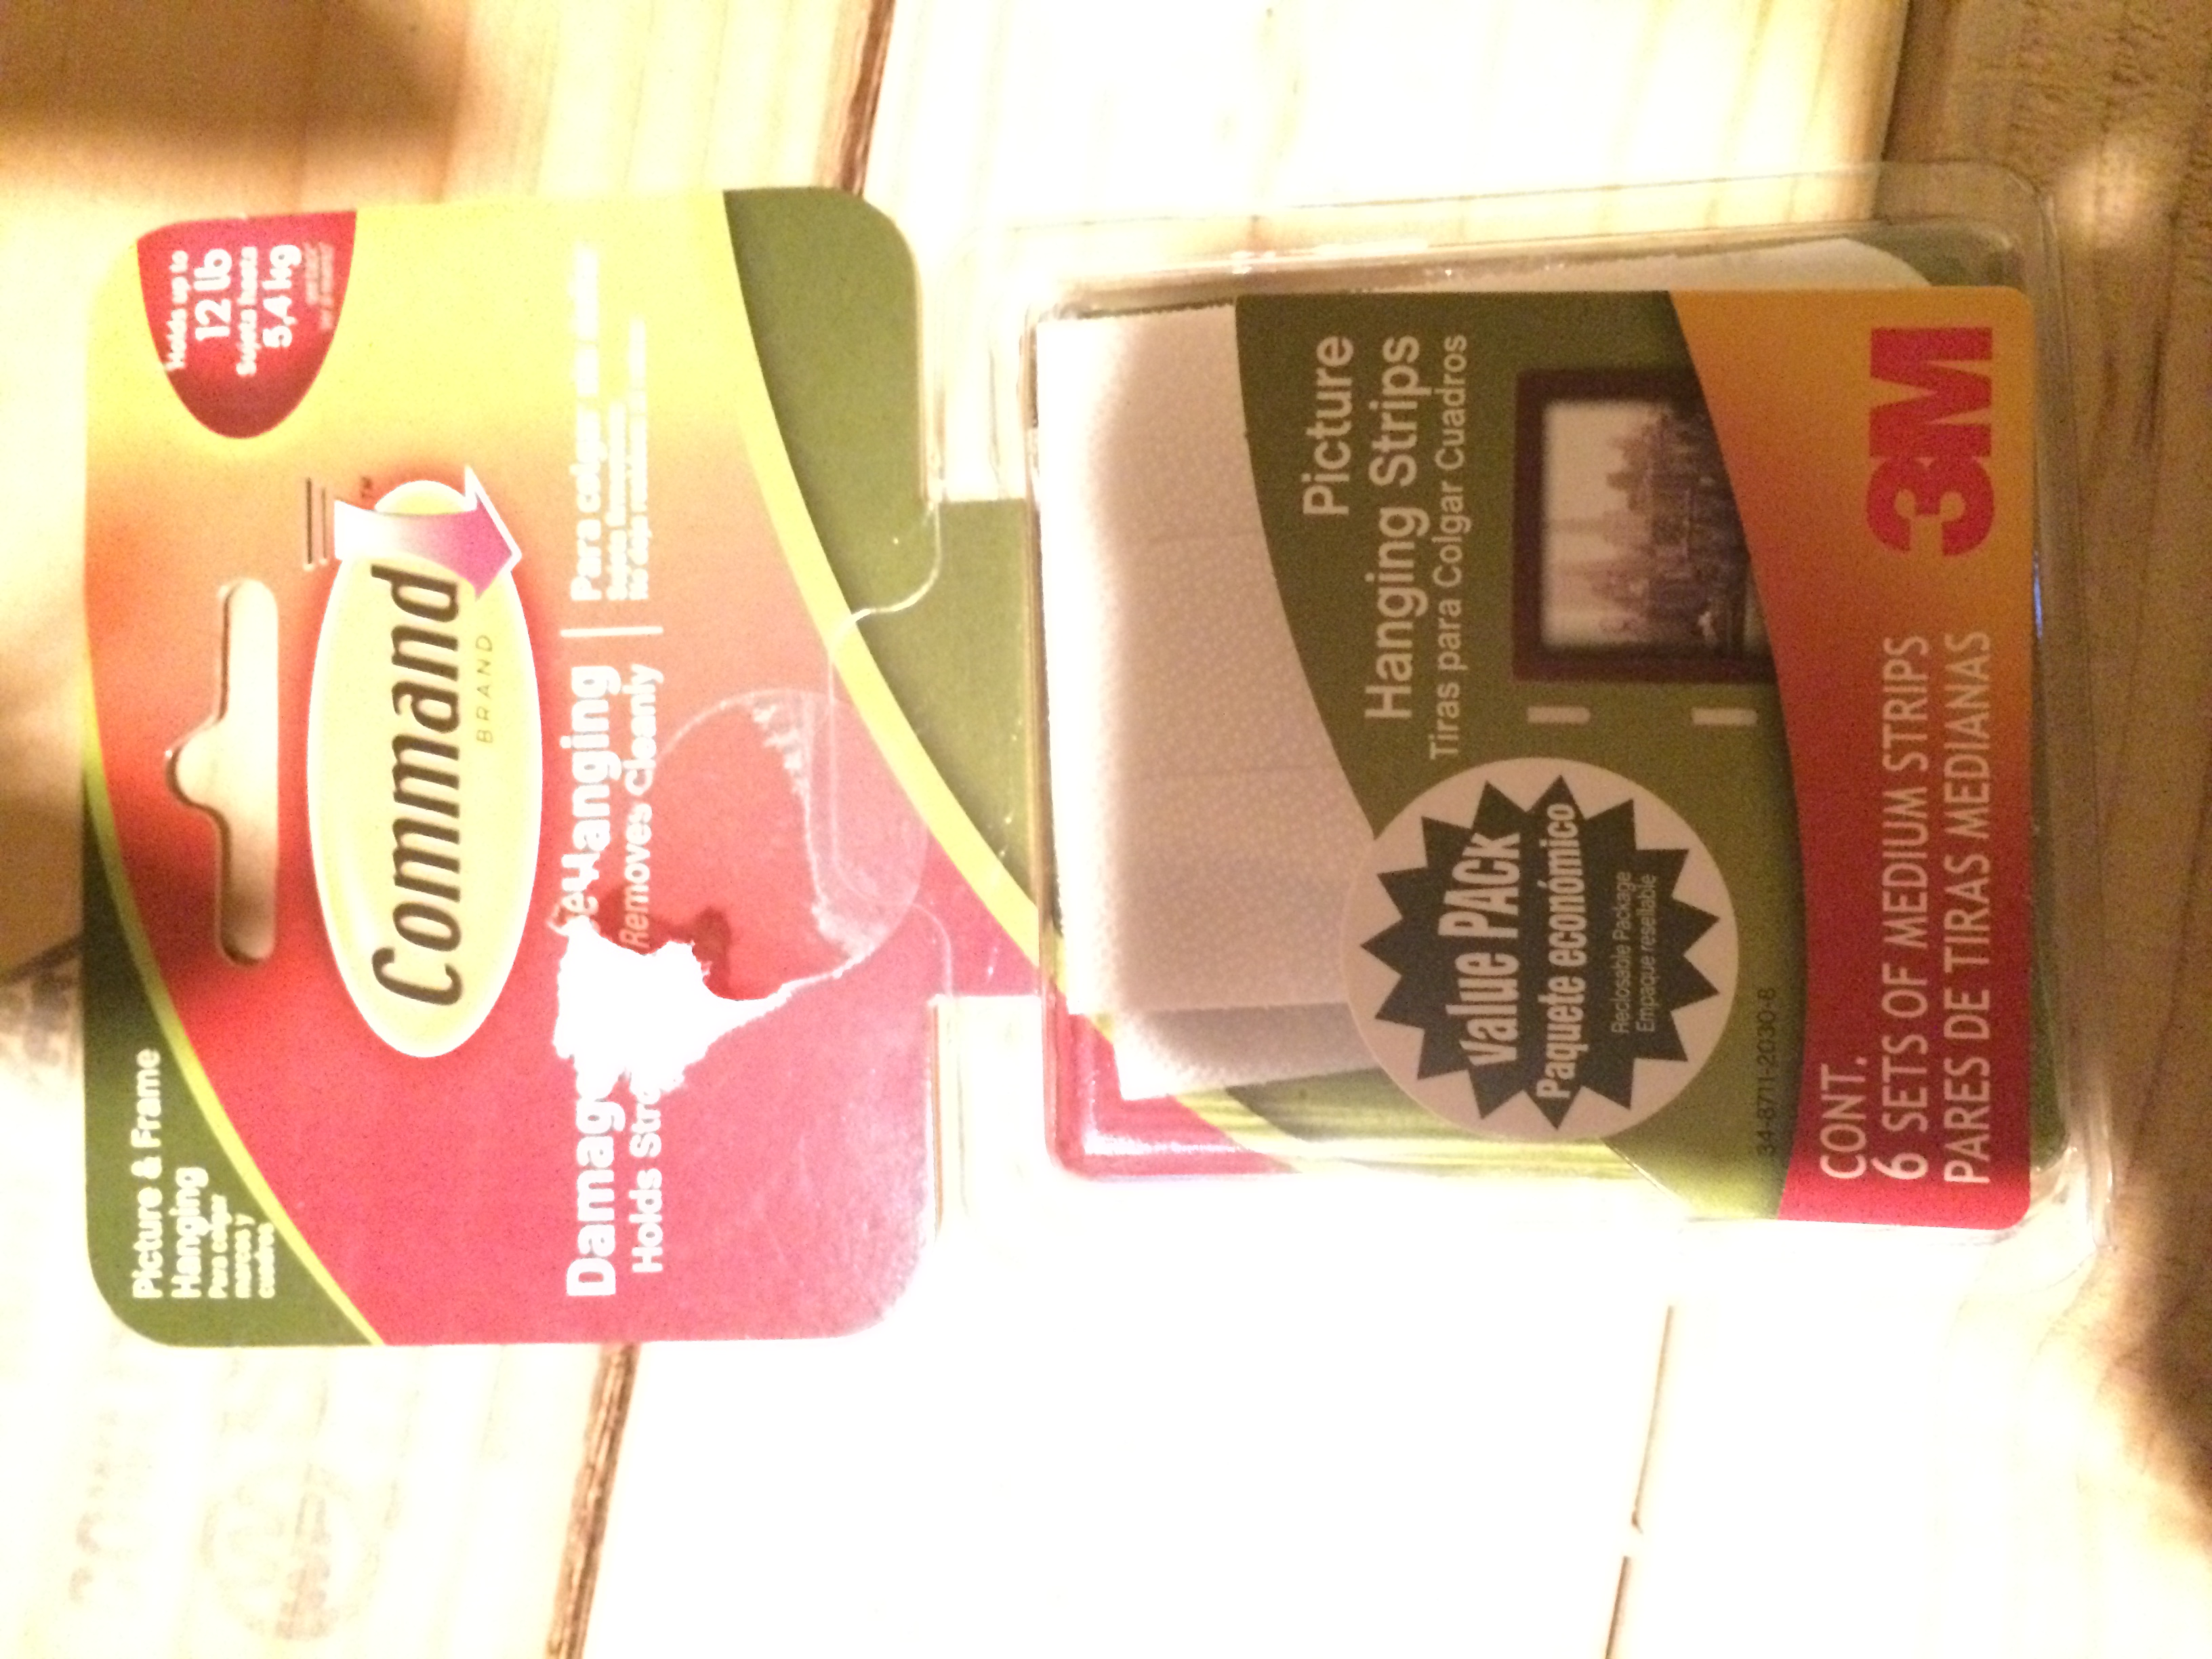
\includegraphics[scale=0.1,angle=270]{images/volume_analysis_setup/IMG_0613.JPG}
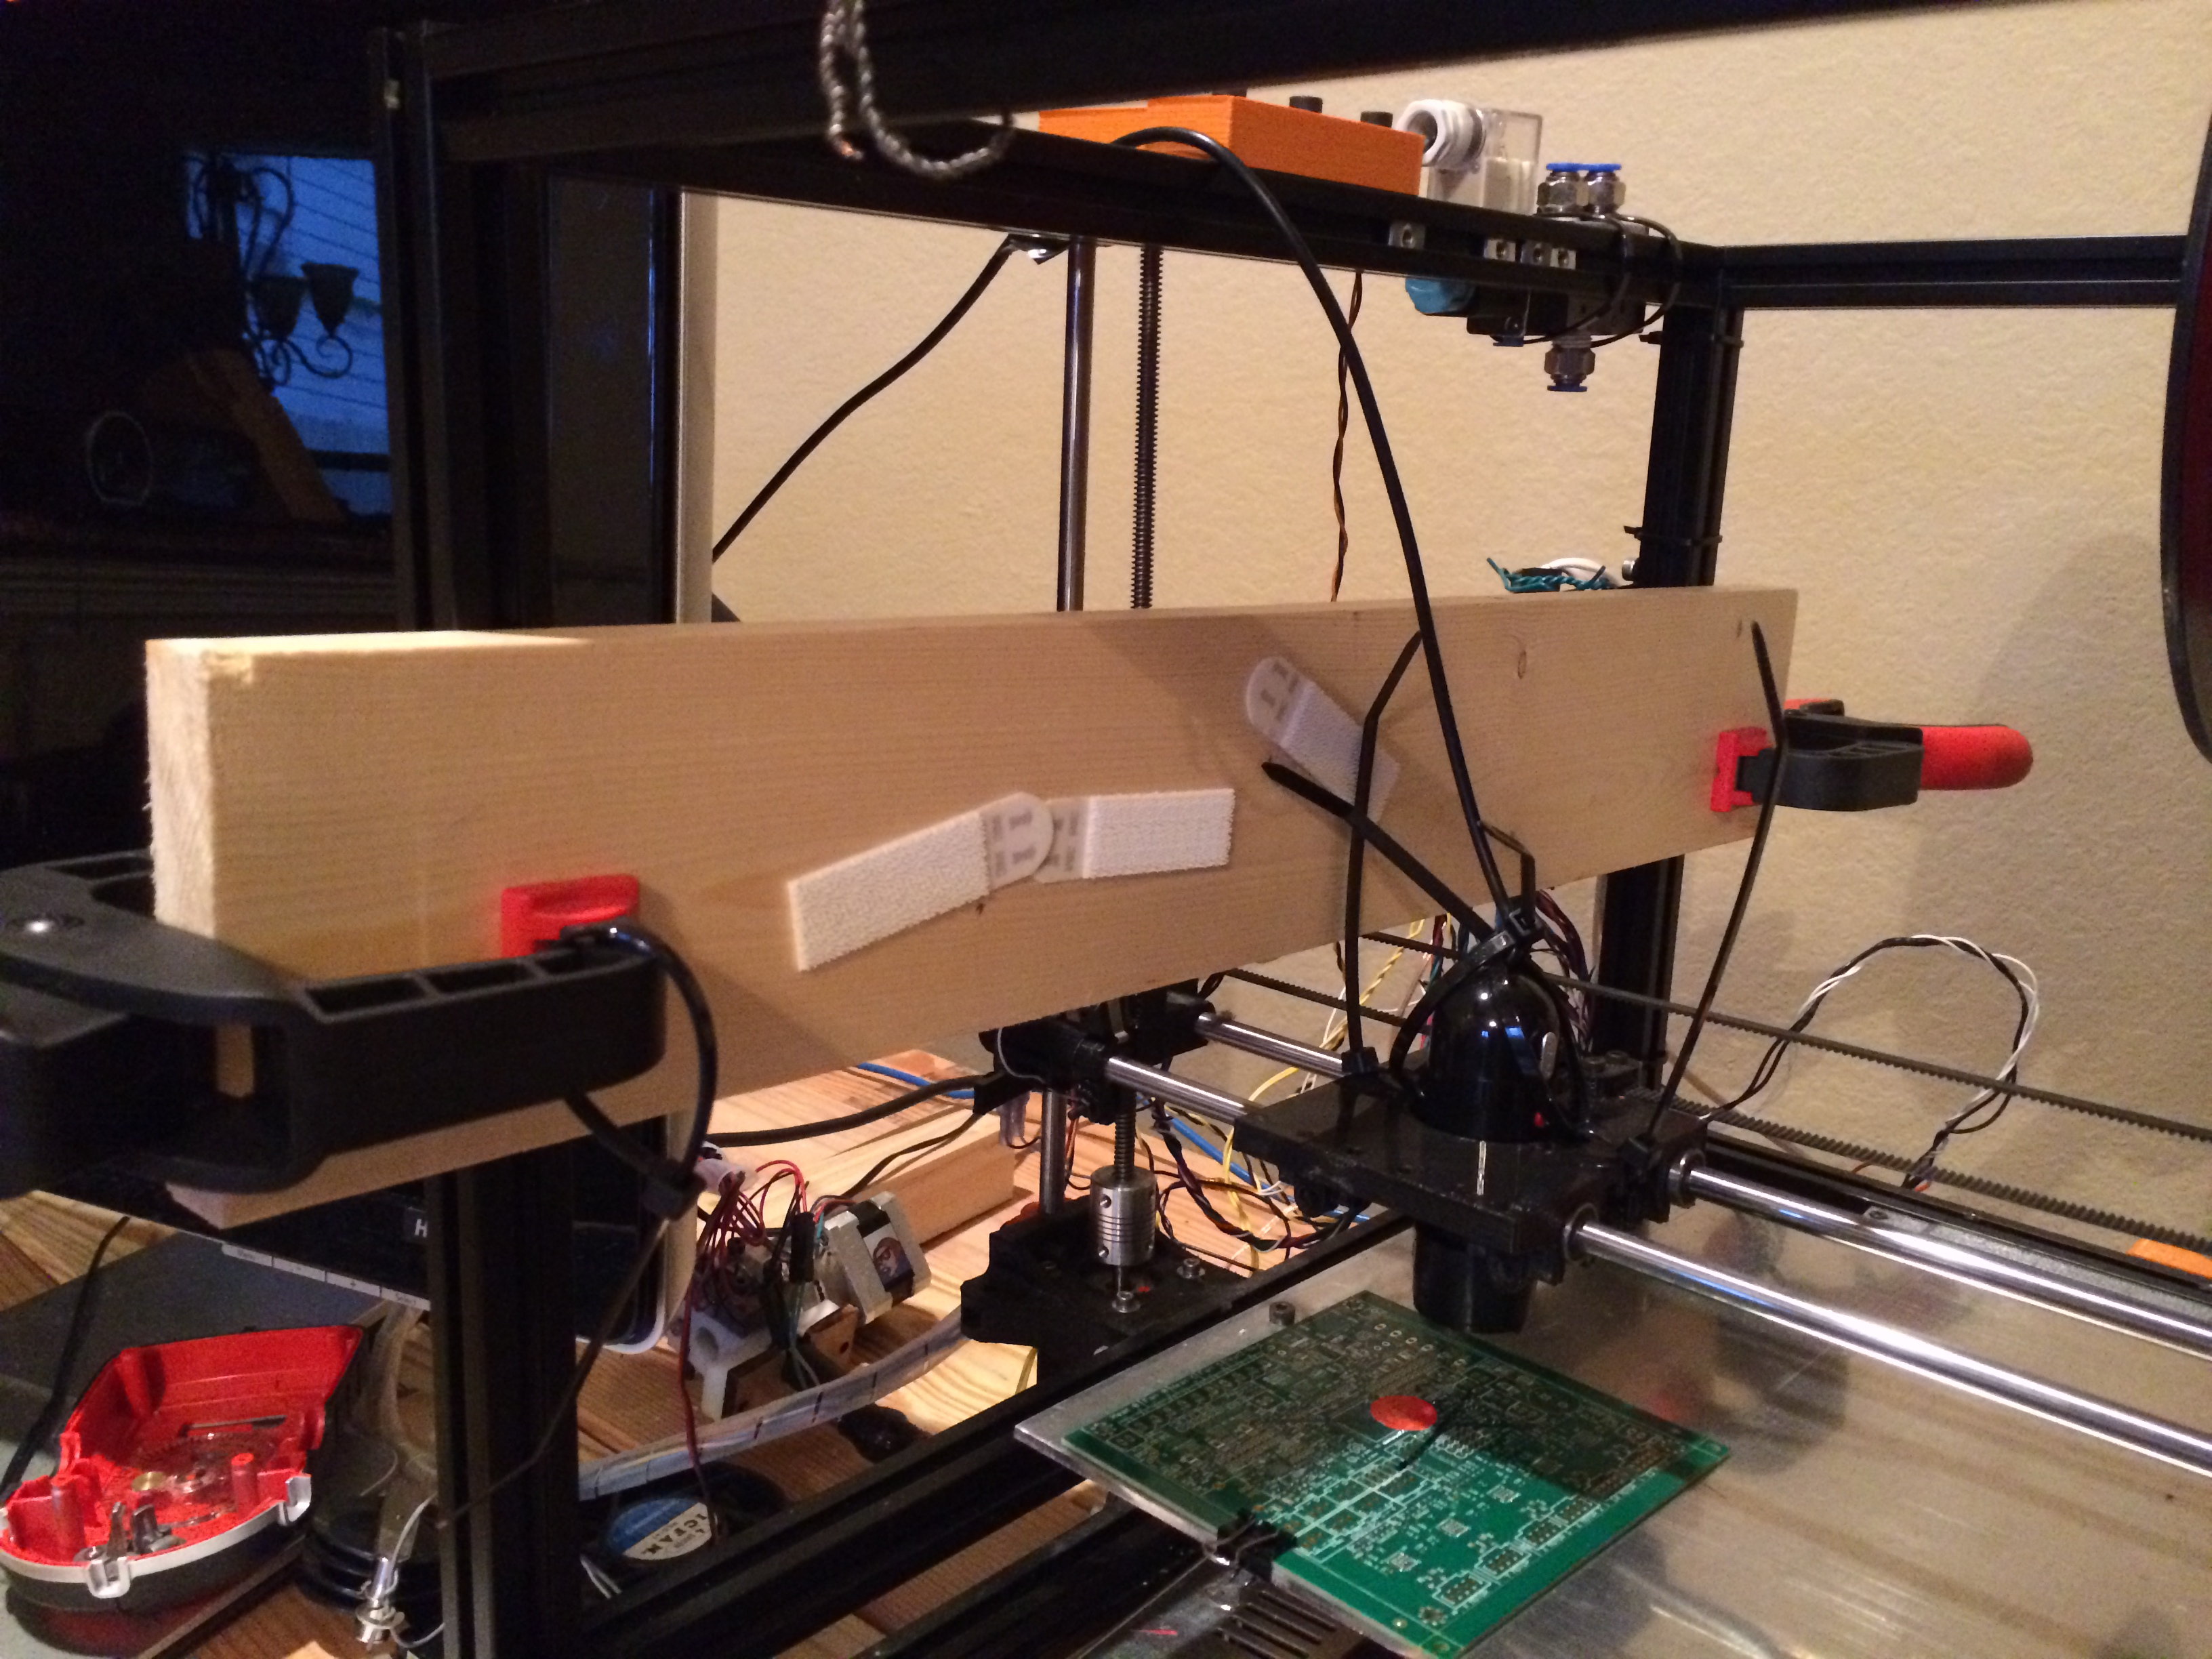
\includegraphics[scale=0.1,angle=270]{images/volume_analysis_setup/IMG_0614.JPG}

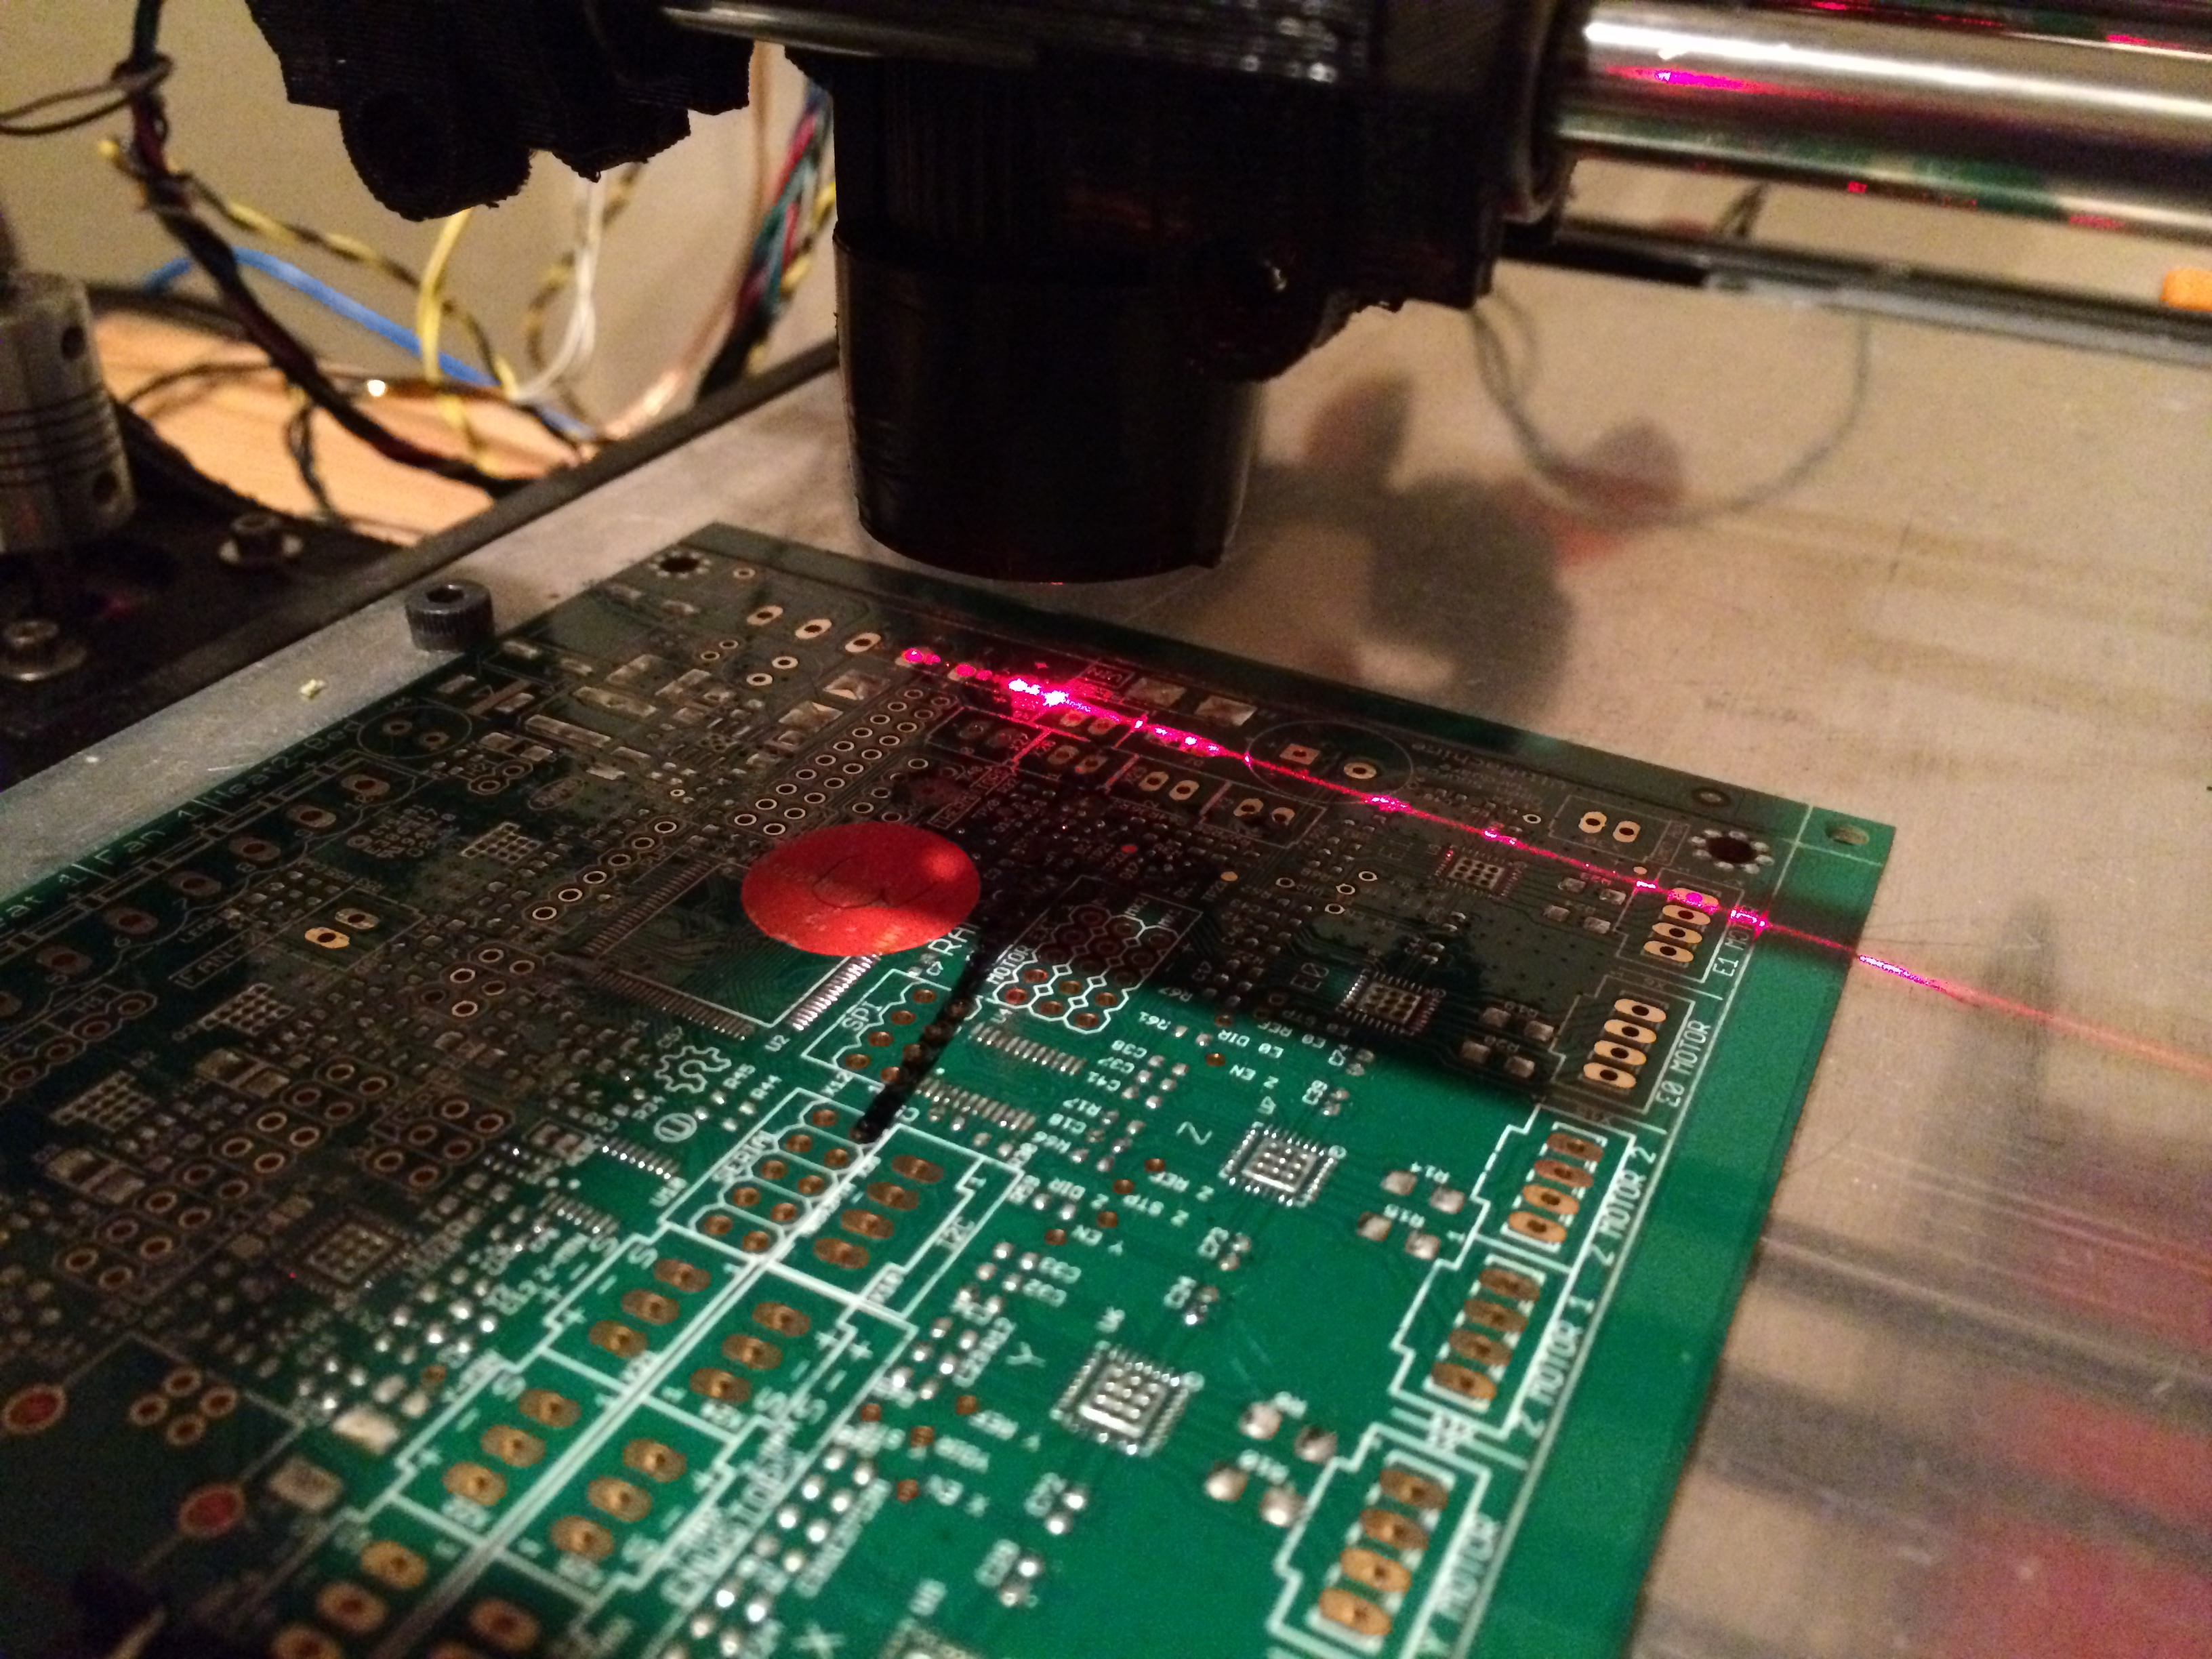
\includegraphics[scale=0.1]{images/volume_analysis_setup/IMG_0606.JPG}

\includegraphics[scale=0.5]{images/volume_analysis_setup/laser-8}
\section{Volume Image Processing}
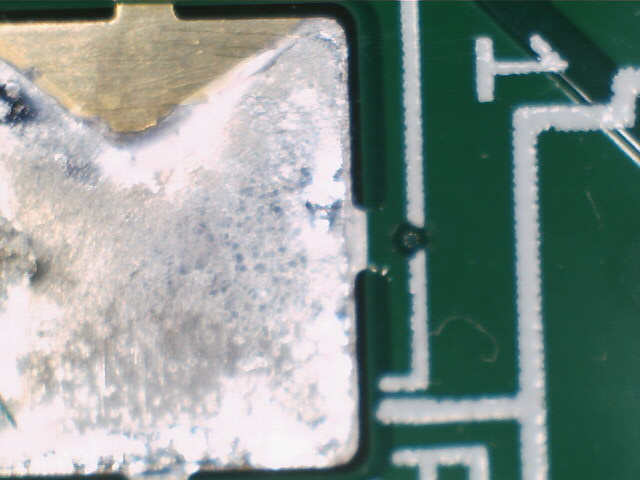
\includegraphics{images/volume_image_processing/led_image.png}
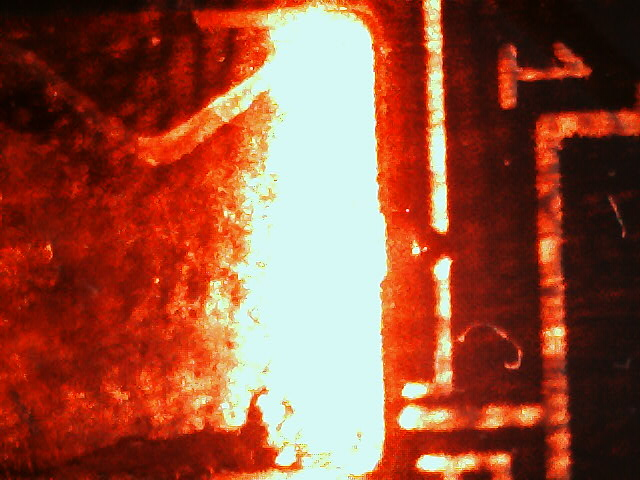
\includegraphics{images/volume_image_processing/laser_image.png}

\includegraphics{images/volume_image_processing/binary_led_image.png}

\includegraphics{images/volume_image_processing/binary_laser_image.png}

\includegraphics{images/volume_image_processing/union_laser_led_binaries.png}

\section{Volume Results}
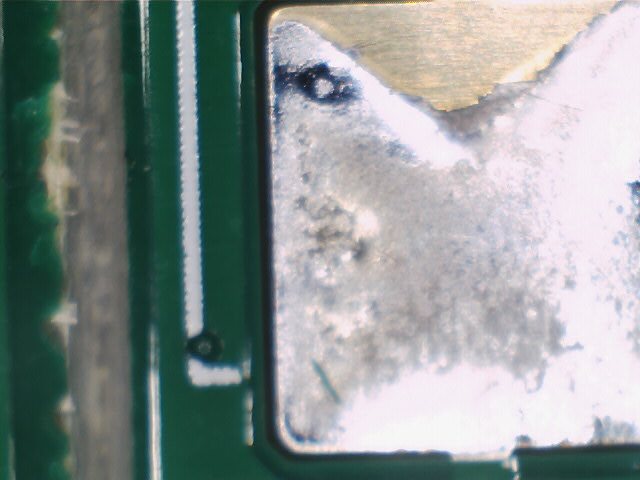
\includegraphics{images/volume_results/solder_led_hole.png}
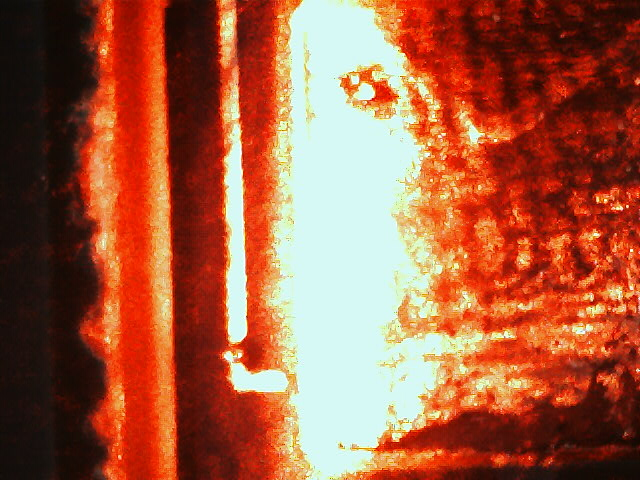
\includegraphics{images/volume_results/solder_laser_hole.png}

\includegraphics{images/volume_results/binary_image_hole.png}




%\begin{abstract}

%\end{abstract}


%\section{Introduction}
%Repeatability and accuracy is essential to PCB manufacturing.  That is why careful inspection %of PCB boards is an integral component of the PCB manufacturing process.  It is also essential %to 3D printing.  As 3D printing technology becomes more common place 

%\paragraph{Outline}
%The remainder of this article is organized as follows.
%Section~\ref{previous work} gives account of previous work.
%Our new and exciting results are described in Section~\ref{results}.
%Finally, Section~\ref{conclusions} gives the conclusions.

%\section{Previous work}\label{previous work}
%A much longer \LaTeXe{} example was written by Gil~\cite{Gil:02}.

%\section{Results}\label{results}
%In this section we describe the results.

%\section{Conclusions}\label{conclusions}
%We worked hard, and achieved very little.

%\bibliographystyle{abbrv}
%\bibliography{main}

\end{document}
